\documentclass[]{article}
\usepackage{lmodern}
\usepackage{amssymb,amsmath}
\usepackage{ifxetex,ifluatex}
\usepackage{fixltx2e} % provides \textsubscript
\ifnum 0\ifxetex 1\fi\ifluatex 1\fi=0 % if pdftex
  \usepackage[T1]{fontenc}
  \usepackage[utf8]{inputenc}
\else % if luatex or xelatex
  \ifxetex
    \usepackage{mathspec}
  \else
    \usepackage{fontspec}
  \fi
  \defaultfontfeatures{Ligatures=TeX,Scale=MatchLowercase}
\fi
% use upquote if available, for straight quotes in verbatim environments
\IfFileExists{upquote.sty}{\usepackage{upquote}}{}
% use microtype if available
\IfFileExists{microtype.sty}{%
\usepackage{microtype}
\UseMicrotypeSet[protrusion]{basicmath} % disable protrusion for tt fonts
}{}
\usepackage[margin=1in]{geometry}
\usepackage{hyperref}
\hypersetup{unicode=true,
            pdftitle={The OmicsPLS R Package},
            pdfauthor={Said el Bouhaddani},
            pdfborder={0 0 0},
            breaklinks=true}
\urlstyle{same}  % don't use monospace font for urls
\usepackage{color}
\usepackage{fancyvrb}
\newcommand{\VerbBar}{|}
\newcommand{\VERB}{\Verb[commandchars=\\\{\}]}
\DefineVerbatimEnvironment{Highlighting}{Verbatim}{commandchars=\\\{\}}
% Add ',fontsize=\small' for more characters per line
\usepackage{framed}
\definecolor{shadecolor}{RGB}{248,248,248}
\newenvironment{Shaded}{\begin{snugshade}}{\end{snugshade}}
\newcommand{\KeywordTok}[1]{\textcolor[rgb]{0.13,0.29,0.53}{\textbf{{#1}}}}
\newcommand{\DataTypeTok}[1]{\textcolor[rgb]{0.13,0.29,0.53}{{#1}}}
\newcommand{\DecValTok}[1]{\textcolor[rgb]{0.00,0.00,0.81}{{#1}}}
\newcommand{\BaseNTok}[1]{\textcolor[rgb]{0.00,0.00,0.81}{{#1}}}
\newcommand{\FloatTok}[1]{\textcolor[rgb]{0.00,0.00,0.81}{{#1}}}
\newcommand{\ConstantTok}[1]{\textcolor[rgb]{0.00,0.00,0.00}{{#1}}}
\newcommand{\CharTok}[1]{\textcolor[rgb]{0.31,0.60,0.02}{{#1}}}
\newcommand{\SpecialCharTok}[1]{\textcolor[rgb]{0.00,0.00,0.00}{{#1}}}
\newcommand{\StringTok}[1]{\textcolor[rgb]{0.31,0.60,0.02}{{#1}}}
\newcommand{\VerbatimStringTok}[1]{\textcolor[rgb]{0.31,0.60,0.02}{{#1}}}
\newcommand{\SpecialStringTok}[1]{\textcolor[rgb]{0.31,0.60,0.02}{{#1}}}
\newcommand{\ImportTok}[1]{{#1}}
\newcommand{\CommentTok}[1]{\textcolor[rgb]{0.56,0.35,0.01}{\textit{{#1}}}}
\newcommand{\DocumentationTok}[1]{\textcolor[rgb]{0.56,0.35,0.01}{\textbf{\textit{{#1}}}}}
\newcommand{\AnnotationTok}[1]{\textcolor[rgb]{0.56,0.35,0.01}{\textbf{\textit{{#1}}}}}
\newcommand{\CommentVarTok}[1]{\textcolor[rgb]{0.56,0.35,0.01}{\textbf{\textit{{#1}}}}}
\newcommand{\OtherTok}[1]{\textcolor[rgb]{0.56,0.35,0.01}{{#1}}}
\newcommand{\FunctionTok}[1]{\textcolor[rgb]{0.00,0.00,0.00}{{#1}}}
\newcommand{\VariableTok}[1]{\textcolor[rgb]{0.00,0.00,0.00}{{#1}}}
\newcommand{\ControlFlowTok}[1]{\textcolor[rgb]{0.13,0.29,0.53}{\textbf{{#1}}}}
\newcommand{\OperatorTok}[1]{\textcolor[rgb]{0.81,0.36,0.00}{\textbf{{#1}}}}
\newcommand{\BuiltInTok}[1]{{#1}}
\newcommand{\ExtensionTok}[1]{{#1}}
\newcommand{\PreprocessorTok}[1]{\textcolor[rgb]{0.56,0.35,0.01}{\textit{{#1}}}}
\newcommand{\AttributeTok}[1]{\textcolor[rgb]{0.77,0.63,0.00}{{#1}}}
\newcommand{\RegionMarkerTok}[1]{{#1}}
\newcommand{\InformationTok}[1]{\textcolor[rgb]{0.56,0.35,0.01}{\textbf{\textit{{#1}}}}}
\newcommand{\WarningTok}[1]{\textcolor[rgb]{0.56,0.35,0.01}{\textbf{\textit{{#1}}}}}
\newcommand{\AlertTok}[1]{\textcolor[rgb]{0.94,0.16,0.16}{{#1}}}
\newcommand{\ErrorTok}[1]{\textcolor[rgb]{0.64,0.00,0.00}{\textbf{{#1}}}}
\newcommand{\NormalTok}[1]{{#1}}
\usepackage{graphicx,grffile}
\makeatletter
\def\maxwidth{\ifdim\Gin@nat@width>\linewidth\linewidth\else\Gin@nat@width\fi}
\def\maxheight{\ifdim\Gin@nat@height>\textheight\textheight\else\Gin@nat@height\fi}
\makeatother
% Scale images if necessary, so that they will not overflow the page
% margins by default, and it is still possible to overwrite the defaults
% using explicit options in \includegraphics[width, height, ...]{}
\setkeys{Gin}{width=\maxwidth,height=\maxheight,keepaspectratio}
\IfFileExists{parskip.sty}{%
\usepackage{parskip}
}{% else
\setlength{\parindent}{0pt}
\setlength{\parskip}{6pt plus 2pt minus 1pt}
}
\setlength{\emergencystretch}{3em}  % prevent overfull lines
\providecommand{\tightlist}{%
  \setlength{\itemsep}{0pt}\setlength{\parskip}{0pt}}
\setcounter{secnumdepth}{0}
% Redefines (sub)paragraphs to behave more like sections
\ifx\paragraph\undefined\else
\let\oldparagraph\paragraph
\renewcommand{\paragraph}[1]{\oldparagraph{#1}\mbox{}}
\fi
\ifx\subparagraph\undefined\else
\let\oldsubparagraph\subparagraph
\renewcommand{\subparagraph}[1]{\oldsubparagraph{#1}\mbox{}}
\fi

%%% Use protect on footnotes to avoid problems with footnotes in titles
\let\rmarkdownfootnote\footnote%
\def\footnote{\protect\rmarkdownfootnote}

%%% Change title format to be more compact
\usepackage{titling}

% Create subtitle command for use in maketitle
\newcommand{\subtitle}[1]{
  \posttitle{
    \begin{center}\large#1\end{center}
    }
}

\setlength{\droptitle}{-2em}
  \title{The OmicsPLS R Package}
  \pretitle{\vspace{\droptitle}\centering\huge}
  \posttitle{\par}
  \author{Said el Bouhaddani}
  \preauthor{\centering\large\emph}
  \postauthor{\par}
  \predate{\centering\large\emph}
  \postdate{\par}
  \date{2016-11-08}


\begin{document}
\maketitle

\section{The OmicsPLS R package}\label{the-omicspls-r-package}

Welcome to the vignette of the O2PLS package for analyzing two Omics
datasets!

Here you can find examples and explanation of the input options and
output objects. As always: help is always found by using the \texttt{?}
operator. Try to type \texttt{?OmicsPLS} for an overview of the package
and \texttt{?o2m} for description of the main fitting function.

\subsection{Background}\label{background}

\subsubsection{The O2PLS method}\label{the-o2pls-method}

The O2PLS method is proposed in (Trygg \& Wold, 2003). It decomposes the
variation of two datasets in three parts:

\begin{itemize}
\tightlist
\item
  A Joint part for \(X\) and \(Y\): \(TW^\top\) and \(UC^\top\),
\item
  A Systematic/Specific/Orthogonal part for \(X\) and \(Y\):
  \(T_\perp W_\perp^\top\) and \(U_\perp C_\perp^\top\),
\item
  A noise part for \(X\) and \(Y\): \(E\) and \(F\).
\end{itemize}

The number of columns in \(T\), \(U\), \(W\) and \(C\) are denoted by as
\(n\) and are referred to as the number of joint components. The number
of columns in \(T_\perp\) and \(W_\perp\) are denoted by as \(n_X\) and
are referred to as the number of \(X\)-specific components. Analoguous
for \(Y\), where we use \(n_Y\) to denote the number of \(Y\)-specific
components. The relation between \(T\) and \(U\) makes the joint part
the joint part: \(U = TB + H\) or \(U = TB'+ H'\). The number of
components \((n, n_X, n_Y)\) are chosen beforehand (e.g.~with
Cross-Validation).

\subsubsection{Cross-Validation}\label{cross-validation}

In cross-validation (CV) one minimizes a certain measure of error over
some parameters that should be determined a priori. In our case we have
three parameters: \((n, n_X, n_Y)\). A popular measure is the prediction
error \(||\hat{Y} - Y||\), where \(\hat{Y}\) is a prediction of \(Y\).
In our case the O2PLS method is symmetric in \(X\) and \(Y\), so we
minimize the sum of the prediction errors:
\(||\hat{X} - X||+||\hat{Y} - Y||\). The idea is to fit O2PLS to our
data \(X\) and \(Y\) and compute the prediction errors for a grid of
values for \(n\), \(n_X\) and \(n_Y\). Here \(n\) should be a positive
integer, and \(n_X\) and \(n_Y\) should be non-negative. The `best'
integers are then the minimizers of the prediction error.

\subsubsection{Proposed cross-validation
approach}\label{proposed-cross-validation-approach}

We proposed an alternative way for choosing the number of components (el
Bouhaddani, 2016). Here we construct a grid of values for \(n\). For
each \(n\) we consider then the \(R^2\) between \(T\) and \(U\) for
different \(n_X\) and \(n_Y\). If \(T\) and \(U\) are contaminated with
data-specific variation the \(R^2\) will be lower. If too many specific
components are removed the \(R^2\) will again be lower. Somewhere in
between is the maximum, with its maximizers \(n_X\) and \(n_Y\). With
these two integers we now compute the prediction error for our \(n\)
that we have kept fixed. This process we repeat for each \(n\) on the
one-dimensional grid and get our maximizers. This can provide a (big)
speed-up and often yields similar values for \((n, n_X, n_Y)\).

\subsection{Installing and loading}\label{installing-and-loading}

The easiest way is to run
\texttt{devtools::install\_github("selbouhaddani/OmicsPLS")}. If this
doesn't work, check if there is a package missing. It imports the
\textbf{ggplot2} and \textbf{parallel} package, so these should be
installed first. If there still is an error, try to download the .tar or
.zip (for Windows) and install offline. These two files can be found
also in the \emph{selbouhaddani/ZippedPackage} repository. Also feel
free to send an email with the error message you are receiving.

The OmicsPLS package is loaded by running \texttt{library(OmicsPLS)}.
Maybe you get a message saying that the \texttt{loadings} object is
masked from \texttt{package::stats}. This basically means that whenever
you type \texttt{loadings} (which is generic), you'll get the
\texttt{loadings.o2m} variant.

\subsection{A first test case}\label{a-first-test-case}

First we generate some data

\begin{Shaded}
\begin{Highlighting}[]
\KeywordTok{set.seed}\NormalTok{(564785412L)}
\NormalTok{X =}\StringTok{ }\KeywordTok{rnorm}\NormalTok{(}\DecValTok{100}\NormalTok{) %*%}\StringTok{ }\KeywordTok{t}\NormalTok{(}\KeywordTok{c}\NormalTok{(}\KeywordTok{rep}\NormalTok{(}\DecValTok{1}\NormalTok{,}\DecValTok{5}\NormalTok{), }\KeywordTok{rep}\NormalTok{(}\DecValTok{0}\NormalTok{,}\DecValTok{45}\NormalTok{))/}\KeywordTok{sqrt}\NormalTok{(}\DecValTok{5}\NormalTok{)) +}\StringTok{ }\CommentTok{# Component 1 = joint}
\StringTok{  }\KeywordTok{rnorm}\NormalTok{(}\DecValTok{100}\NormalTok{) %*%}\StringTok{ }\KeywordTok{t}\NormalTok{(}\KeywordTok{c}\NormalTok{(}\KeywordTok{rep}\NormalTok{(}\DecValTok{0}\NormalTok{,}\DecValTok{45}\NormalTok{), }\KeywordTok{rep}\NormalTok{(}\DecValTok{1}\NormalTok{,}\DecValTok{5}\NormalTok{))/}\KeywordTok{sqrt}\NormalTok{(}\DecValTok{5}\NormalTok{)) }\CommentTok{# Component 2 = specific}
\NormalTok{Y =}\StringTok{ }\NormalTok{X[,}\KeywordTok{c}\NormalTok{(}\DecValTok{6}\NormalTok{:}\DecValTok{25}\NormalTok{, }\DecValTok{1}\NormalTok{:}\DecValTok{5}\NormalTok{, }\DecValTok{26}\NormalTok{:}\DecValTok{45}\NormalTok{)] }\CommentTok{# Reorder columns of X and leave out last 5}
\NormalTok{X =}\StringTok{ }\NormalTok{X +}\StringTok{ }\KeywordTok{matrix}\NormalTok{(}\KeywordTok{rnorm}\NormalTok{(}\DecValTok{100}\NormalTok{*}\DecValTok{50}\NormalTok{), }\DataTypeTok{nrow=}\DecValTok{100}\NormalTok{) }\CommentTok{# add noise}
\NormalTok{Y =}\StringTok{ }\NormalTok{Y +}\StringTok{ }\KeywordTok{matrix}\NormalTok{(}\KeywordTok{rnorm}\NormalTok{(}\DecValTok{100}\NormalTok{*}\DecValTok{45}\NormalTok{), }\DataTypeTok{nrow=}\DecValTok{100}\NormalTok{) }\CommentTok{# add noise}

\NormalTok{X =}\StringTok{ }\KeywordTok{scale}\NormalTok{(X, }\DataTypeTok{scale=}\NormalTok{F)}
\NormalTok{Y =}\StringTok{ }\KeywordTok{scale}\NormalTok{(Y, }\DataTypeTok{scale=}\NormalTok{F)}
\end{Highlighting}
\end{Shaded}

Now \texttt{X} has 100 rows and 50 columns while \texttt{Y} has 100 rows
and 45 columns. We used two latent components in \(X\), which are hidden
in the first five and last five variables. The first five variables are
also present in \(Y_{20}\) to \(Y_{25}\). We add noise so we do not
exactly observe the latent structures.

We will use the \texttt{gplots} package to create heatmaps of
correlations.

\begin{Shaded}
\begin{Highlighting}[]
\KeywordTok{try}\NormalTok{(}
  \NormalTok{gplots::}\KeywordTok{heatmap.2}\NormalTok{(}\KeywordTok{cor}\NormalTok{(X,Y), }\DataTypeTok{Rowv=}\NormalTok{F,}\DataTypeTok{Colv=}\NormalTok{F, }\DataTypeTok{col=}\NormalTok{gplots::}\KeywordTok{bluered}\NormalTok{(}\DecValTok{100}\NormalTok{)),}
  \DataTypeTok{silent =} \OtherTok{TRUE}\NormalTok{)}
\end{Highlighting}
\end{Shaded}

\begin{verbatim}
## Warning in gplots::heatmap.2(cor(X, Y), Rowv = F, Colv = F, col =
## gplots::bluered(100)): Discrepancy: Rowv is FALSE, while dendrogram is
## `both'. Omitting row dendogram.
\end{verbatim}

\begin{verbatim}
## Warning in gplots::heatmap.2(cor(X, Y), Rowv = F, Colv = F, col =
## gplots::bluered(100)): Discrepancy: Colv is FALSE, while dendrogram is
## `column'. Omitting column dendogram.
\end{verbatim}

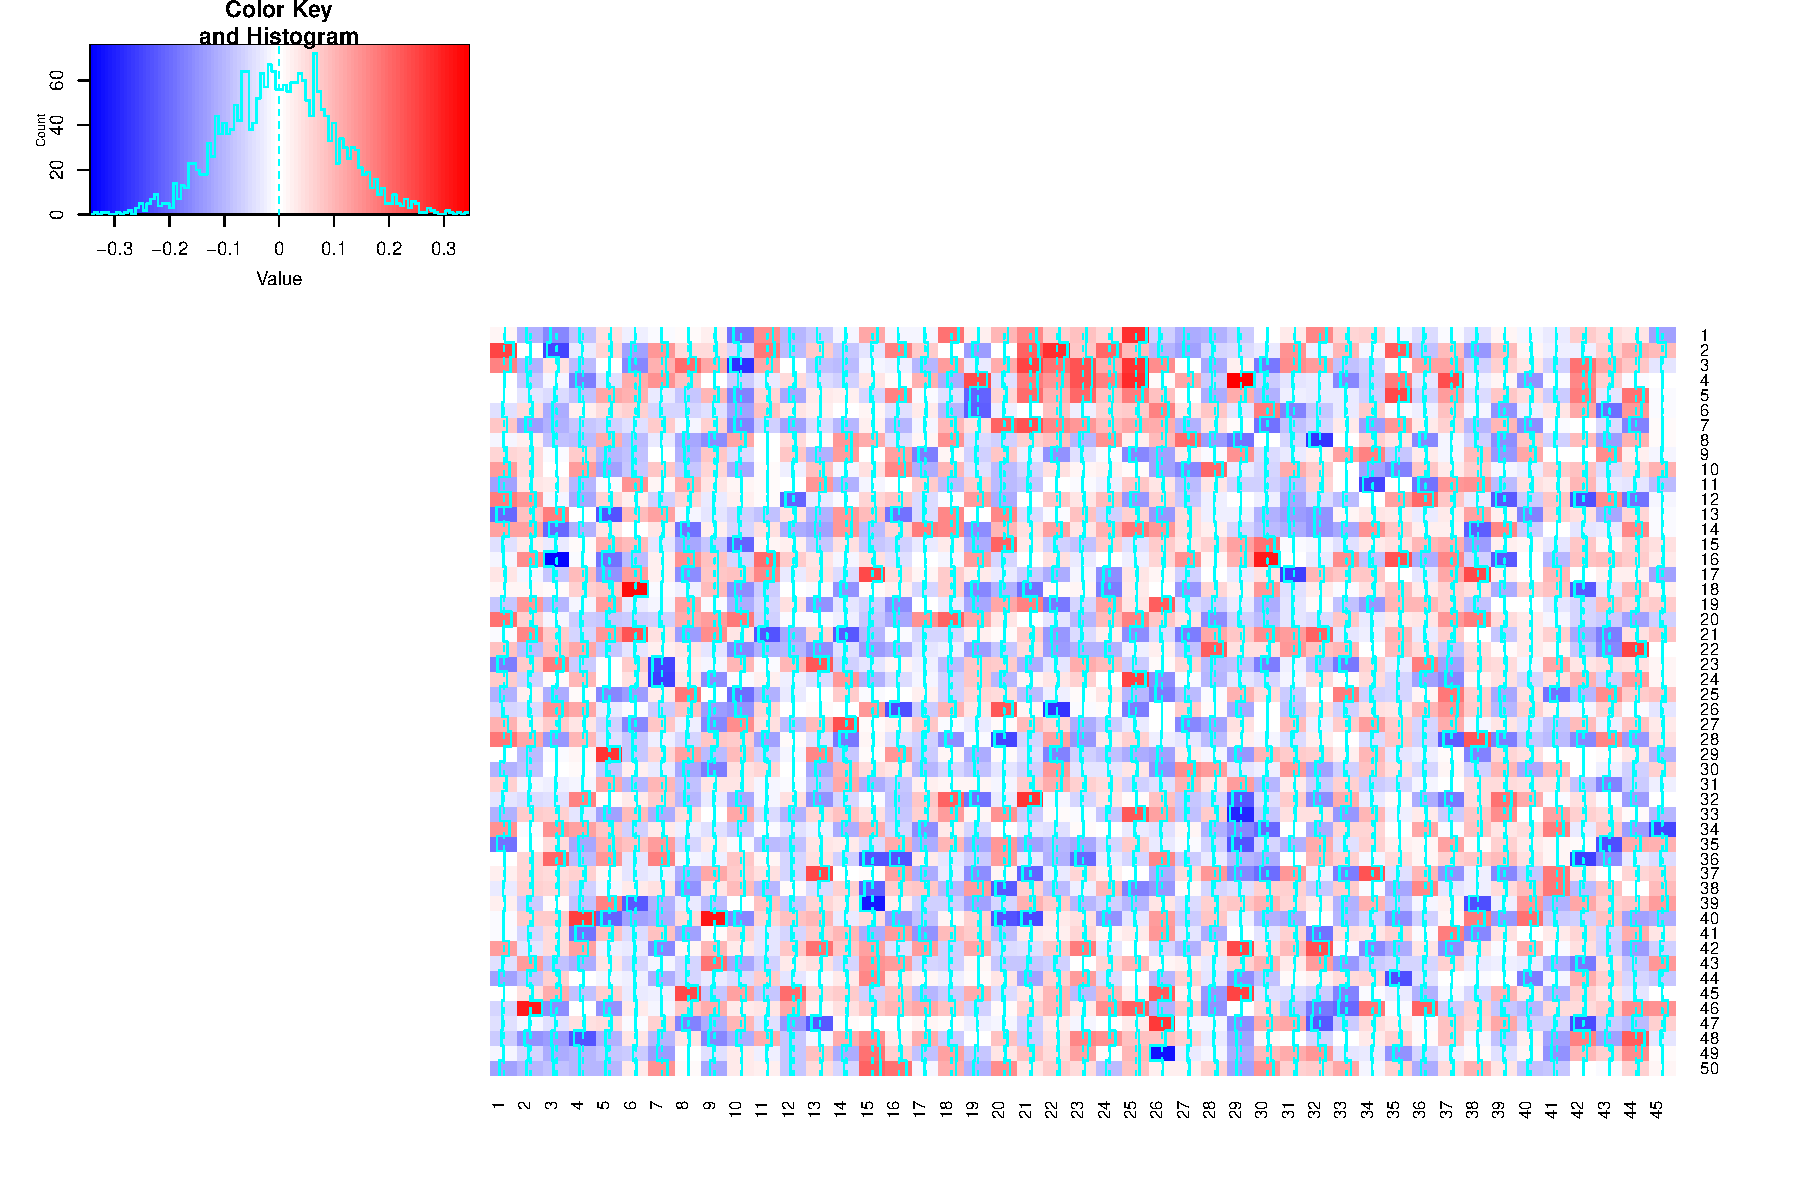
\includegraphics{Figs/unnamed-chunk-2-1.pdf} It is difficult to see
where the correlated part lies. We will try to find out with O2PLS.
First we need to determine the number of components.

\begin{Shaded}
\begin{Highlighting}[]
\KeywordTok{library}\NormalTok{(OmicsPLS)}
\KeywordTok{set.seed}\NormalTok{(1221L)}
\KeywordTok{crossval_o2m_adjR2}\NormalTok{(X, Y, }\DecValTok{1}\NormalTok{:}\DecValTok{3}\NormalTok{, }\DecValTok{0}\NormalTok{:}\DecValTok{3}\NormalTok{, }\DecValTok{0}\NormalTok{:}\DecValTok{3}\NormalTok{, }\DataTypeTok{nr_folds =} \DecValTok{2}\NormalTok{)}
\end{Highlighting}
\end{Shaded}

\begin{verbatim}
## minimum is at n = 1
\end{verbatim}

\begin{verbatim}
## Elapsed time: 0.55 sec
\end{verbatim}

\begin{verbatim}
##        MSE n nx ny
## 1 2.030027 1  1  1
## 2 2.053605 2  3  3
## 3 2.083403 3  3  3
\end{verbatim}

\begin{Shaded}
\begin{Highlighting}[]
\KeywordTok{crossval_o2m}\NormalTok{(X, Y, }\DecValTok{1}\NormalTok{:}\DecValTok{3}\NormalTok{, }\DecValTok{0}\NormalTok{:}\DecValTok{3}\NormalTok{, }\DecValTok{0}\NormalTok{:}\DecValTok{3}\NormalTok{, }\DataTypeTok{nr_folds =} \DecValTok{10}\NormalTok{)}
\end{Highlighting}
\end{Shaded}

\begin{verbatim}
## *******************
## Elapsed time: 3.76 sec
## *******
## Minimal 10-CV error is at ax=0 ay=1 a=1 
## *******
## Minimum is 2.022266 
## *******************
\end{verbatim}

The alternative cross-validation suggests one component in all parts.
The full cross-validation suggests one joint and one \(X\)-specific
component. Although the full CV got it right, the alternative yielded
similar answers in much less CPU time (a factor of ten faster). This is
partly because we use more folds, but decreasing the number of folds to
two yielded unreliable results for the full CV.

We now fit the O2PLS model.

\begin{Shaded}
\begin{Highlighting}[]
\NormalTok{fit0 =}\StringTok{ }\KeywordTok{o2m}\NormalTok{(X, Y, }\DecValTok{1}\NormalTok{, }\DecValTok{1}\NormalTok{, }\DecValTok{0}\NormalTok{)}
\NormalTok{fit0}
\end{Highlighting}
\end{Shaded}

\begin{verbatim}
## O2PLS fit 
## with 1 joint components  
## and  1 orthogonal components in X 
## and  0 orthogonal components in Y 
## Elapsed time: 0 sec
\end{verbatim}

\begin{Shaded}
\begin{Highlighting}[]
\KeywordTok{summary}\NormalTok{(fit0)}
\end{Highlighting}
\end{Shaded}

\begin{verbatim}
## 
## *** Summary of the O2PLS fit *** 
## 
## -  Call: o2m(X = X, Y = Y, n = 1, nx = 1, ny = 0) 
## 
## -  Modeled variation
## -- Total variation:
## in X: 5100.552 
## in Y: 4576.141 
## 
## -- Joint, Orthogonal and Noise as proportions:
## 
##            data X data Y
## Joint       0.040  0.054
## Orthogonal  0.042  0.000
## Noise       0.918  0.946
## 
## -- Predictable variation in Y-joint part by X-joint part:
## Variation in Yhat relative to U: 0.693 
## -- Predictable variation in X-joint part by Y-joint part:
## Variation in Xhat relative to T: 0.693 
## 
## -- Variances per component:
## 
##          Comp 1
## X joint 206.273
## Y joint 247.776
## 
##         Comp 1
## X Orth 212.371
## 
## 
## -  Coefficient in 'U = T B_T + H_U' model:
## -- Diagonal elements of B_T =
##  0.912
\end{verbatim}

We can see that there is a lot of noise (92\% and 95\%), and only about
5\% joint variation. However relative to this variation, 69\% is
predictable. To see which variables induce the joint variation, we plot
the joint loadings of \(X\) and \(Y\).

\begin{Shaded}
\begin{Highlighting}[]
\KeywordTok{plot}\NormalTok{(fit0)}
\end{Highlighting}
\end{Shaded}

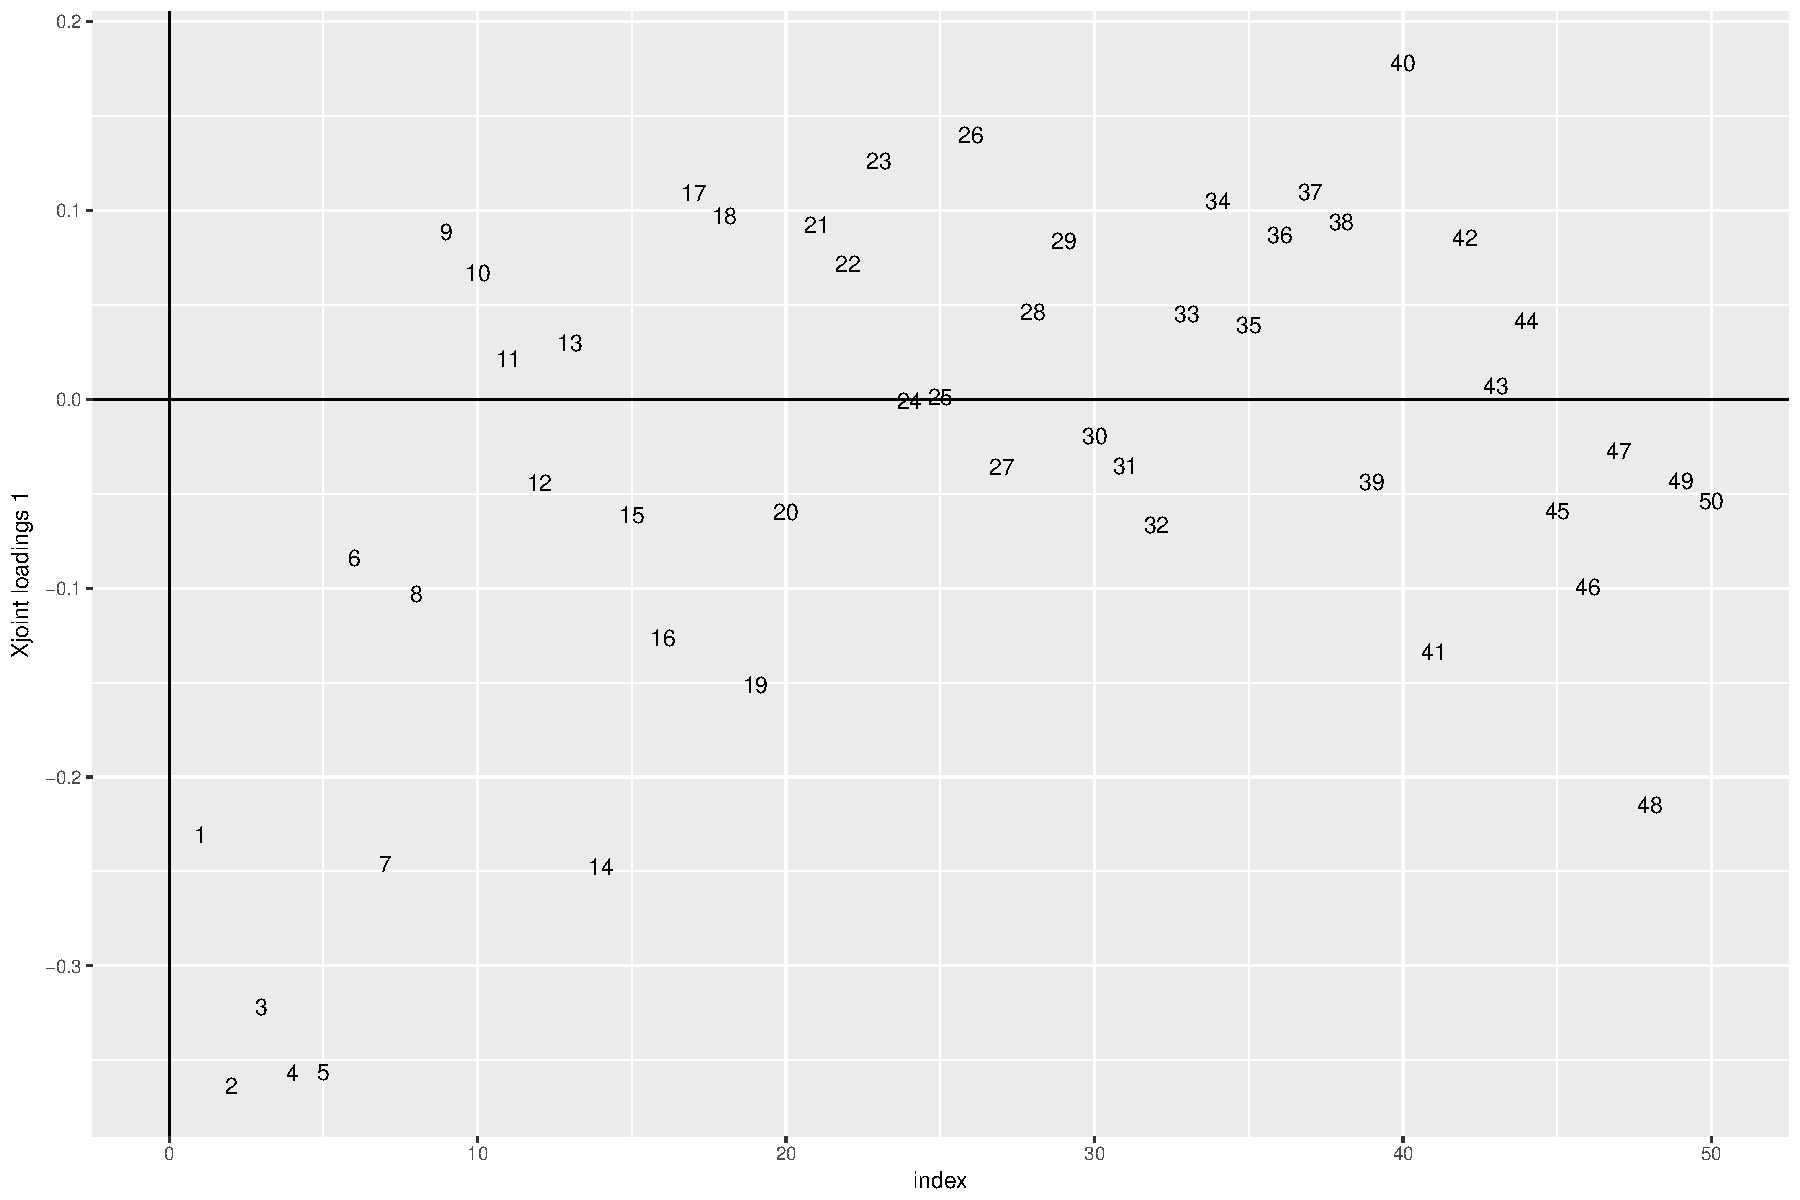
\includegraphics{Figs/unnamed-chunk-5-1.pdf}

\begin{Shaded}
\begin{Highlighting}[]
\KeywordTok{plot}\NormalTok{(fit0, }\StringTok{"Yj"}\NormalTok{)}
\end{Highlighting}
\end{Shaded}

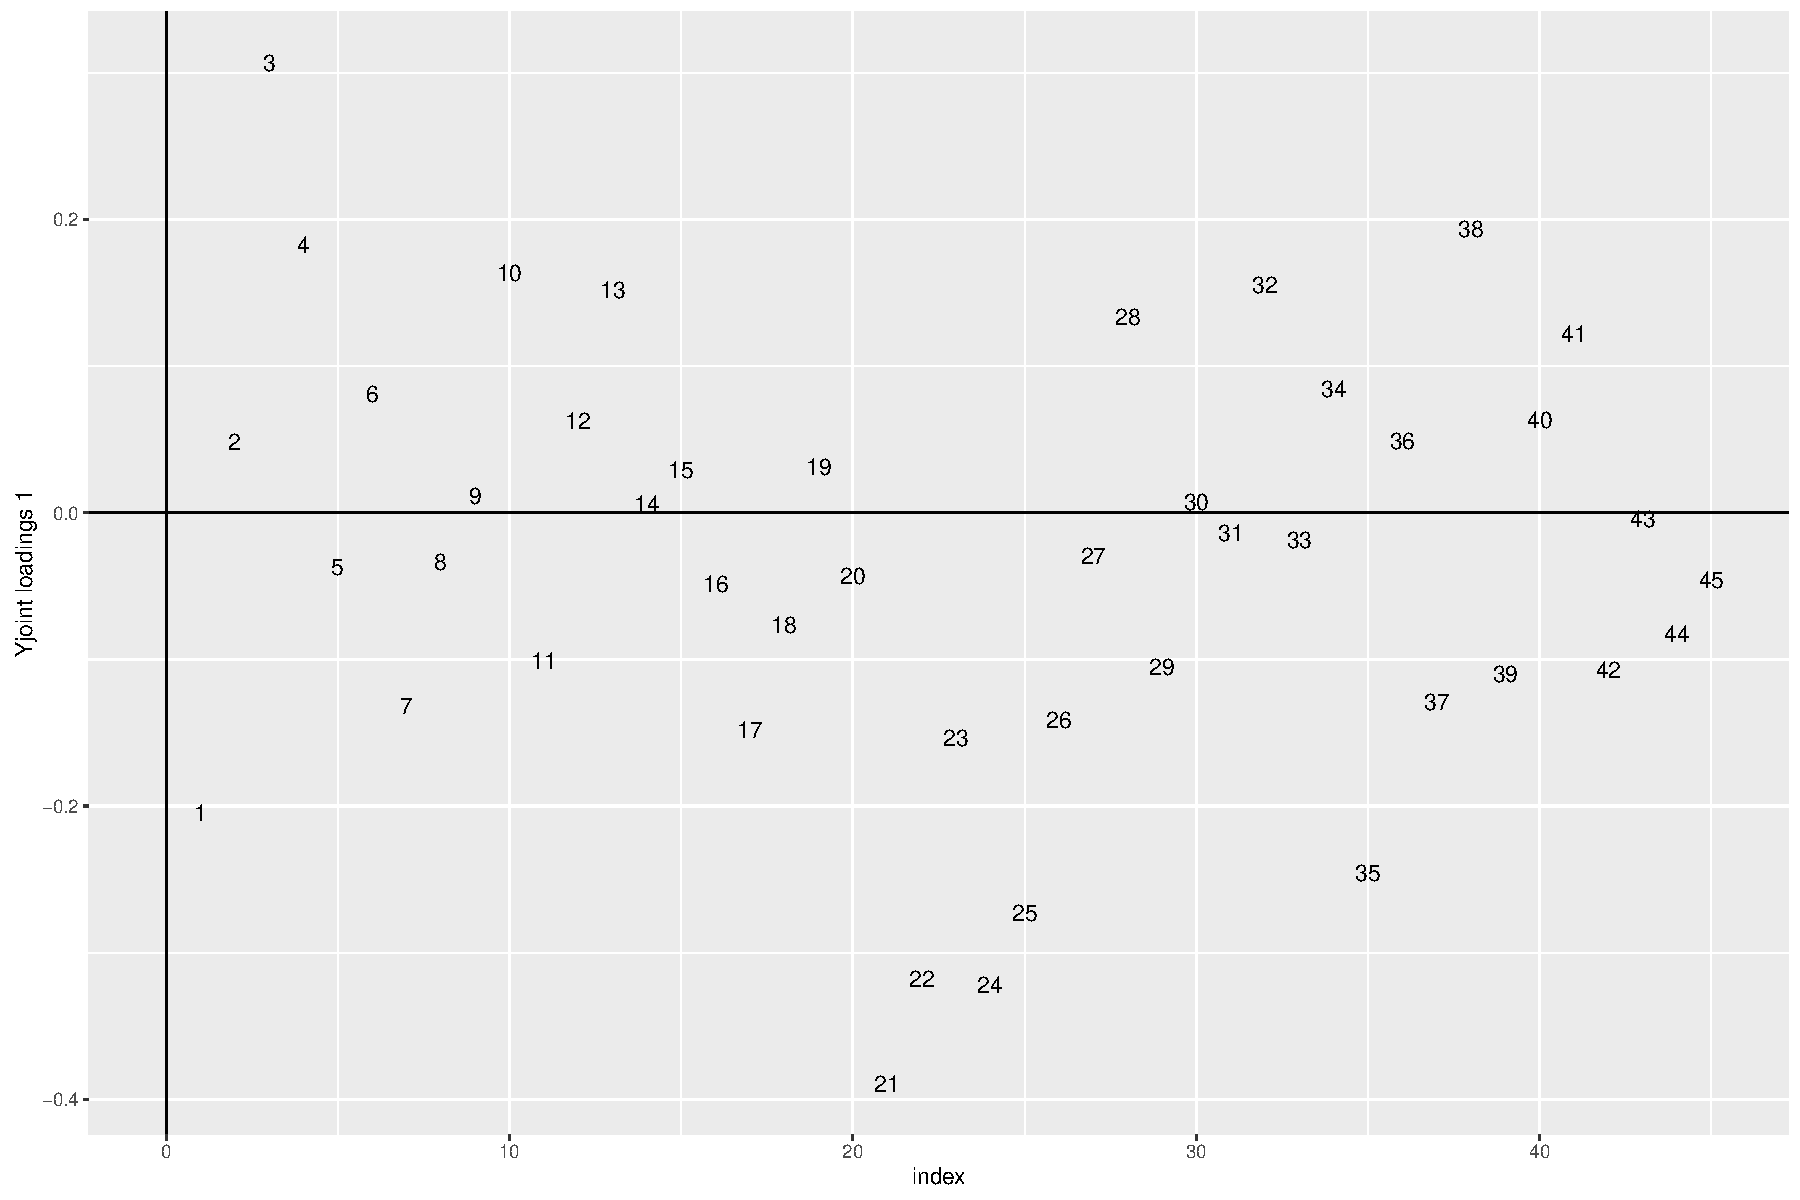
\includegraphics{Figs/unnamed-chunk-5-2.pdf} We see that more or less
the first five \(X\) variables and columns 21 to 25 of \(Y\) have high
absolute loading values.

The \(X\)-specific loadings are not recovered unfortunately, probably
due to the high noise level.

\begin{Shaded}
\begin{Highlighting}[]
\KeywordTok{plot}\NormalTok{(fit0, }\StringTok{"Xo"}\NormalTok{)}
\end{Highlighting}
\end{Shaded}

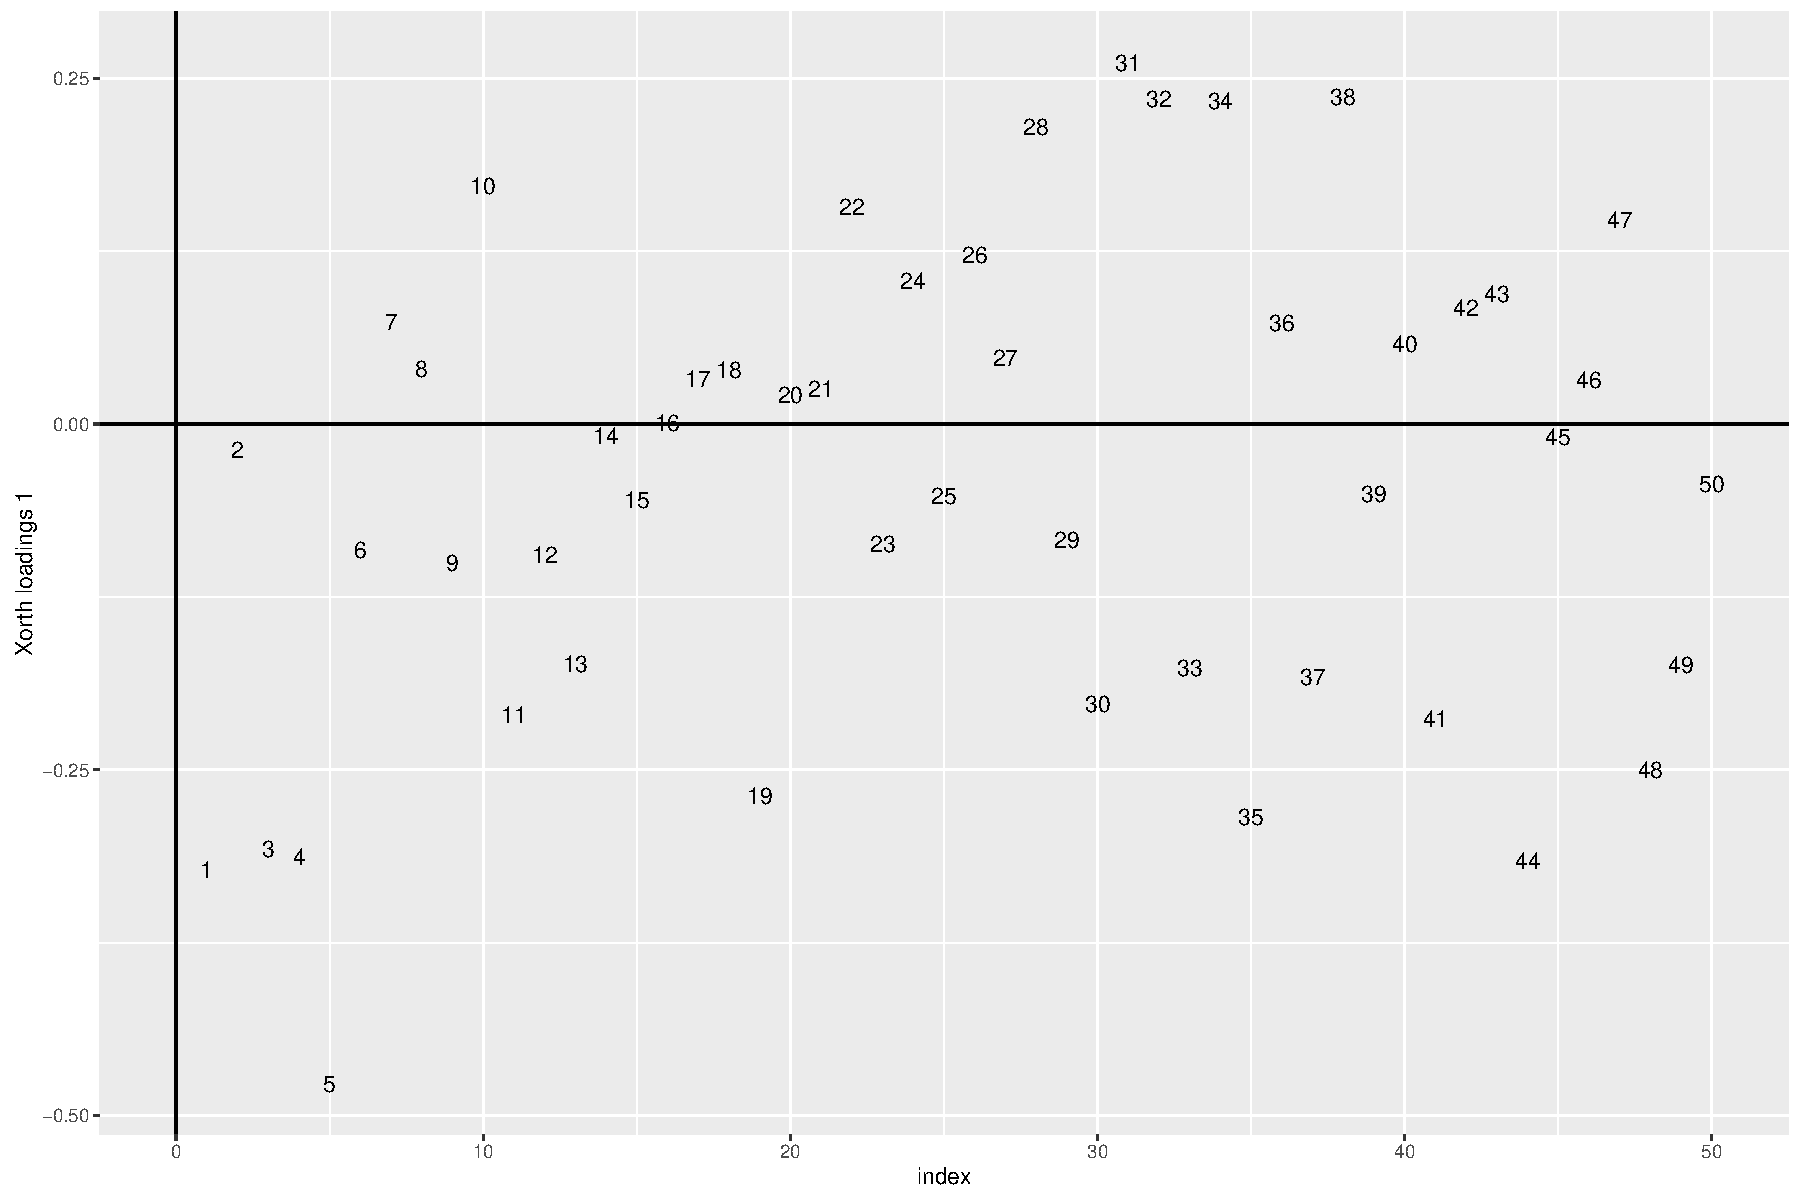
\includegraphics{Figs/unnamed-chunk-6-1.pdf}

\subsection{Real data example}\label{real-data-example}

First we define a function to pick only the top \texttt{100*prop}
percent of the genes that have highest expression level, intersected
with the top \texttt{100*prop} percent with highest Inter Quantile
Range.

\begin{Shaded}
\begin{Highlighting}[]
\NormalTok{filter_rna <-}\StringTok{ }\NormalTok{function(}\DataTypeTok{rna=}\NormalTok{rna, }\DataTypeTok{prop =} \FloatTok{0.75}\NormalTok{)\{}
  \CommentTok{#first, calculate the maximum of gene expression per each gene and take the quantiles, we are interested in top 25% of the gene expressions}
  \NormalTok{maxGE <-}\StringTok{ }\KeywordTok{apply}\NormalTok{(rna, }\DecValTok{2}\NormalTok{, max)}
  \NormalTok{propGEmax <-}\StringTok{ }\KeywordTok{quantile}\NormalTok{(maxGE, prop)}
  \CommentTok{#next, take the IQR of each gene, to capture the variability and check the top 25% genes according to the size of IQR}
  \NormalTok{IQRGE <-}\StringTok{ }\KeywordTok{apply}\NormalTok{(rna, }\DecValTok{2}\NormalTok{, IQR, }\DataTypeTok{na.rm=}\OtherTok{TRUE}\NormalTok{) }
  \NormalTok{propGEIQR <-}\StringTok{ }\KeywordTok{quantile}\NormalTok{(IQRGE, prop)}
  \CommentTok{#selected genes/probes is the intersection of the two previous sets}
  \NormalTok{filter2 <-}\StringTok{ }\NormalTok{(}\KeywordTok{intersect}\NormalTok{(}\KeywordTok{which}\NormalTok{(maxGE>}\StringTok{ }\NormalTok{propGEmax), }\KeywordTok{which}\NormalTok{(IQRGE>}\StringTok{ }\NormalTok{propGEIQR)))}
  \KeywordTok{return}\NormalTok{(filter2)}
\NormalTok{\}}
\end{Highlighting}
\end{Shaded}

\subsubsection{Load in the data}\label{load-in-the-data}

\textbf{Packages needed}

\begin{itemize}
\tightlist
\item
  \texttt{install.packages("data.table")}
\end{itemize}

Now we load in the data, assumed it is downloaded and stored on disk,
and prepare it in the right format (samples as rows and genes as
columns) and give the rows and columns the right names. We use the
package \texttt{data.table} as this reads in large data sets much
faster.

\begin{Shaded}
\begin{Highlighting}[]
\KeywordTok{set.seed}\NormalTok{(}\DecValTok{31}\NormalTok{*}\DecValTok{12}\NormalTok{*}\DecValTok{2016}\NormalTok{)}
\NormalTok{rna0 <-}\StringTok{ }\NormalTok{data.table::}\KeywordTok{fread}\NormalTok{(}\StringTok{"C:/Users/selbouhaddani/MEGANZ/Downloads/O2PLS_BiB/test.tab"}\NormalTok{,}\DataTypeTok{header=}\NormalTok{T, }\DataTypeTok{sep=}\StringTok{'}\CharTok{\textbackslash{}t}\StringTok{'}\NormalTok{)}
\end{Highlighting}
\end{Shaded}

\begin{verbatim}
## 
Read 28.2% of 35420 rows
Read 56.5% of 35420 rows
Read 84.7% of 35420 rows
Read 35420 rows and 519 (of 519) columns from 0.289 GB file in 00:00:08
\end{verbatim}

\begin{Shaded}
\begin{Highlighting}[]
\NormalTok{rna1 <-}\StringTok{ }\KeywordTok{t}\NormalTok{(}\KeywordTok{as.data.frame.matrix}\NormalTok{(rna0[-}\DecValTok{1}\NormalTok{,-}\DecValTok{1}\NormalTok{,}\DataTypeTok{with=}\NormalTok{F]))}
\NormalTok{rna2 <-}\StringTok{ }\KeywordTok{matrix}\NormalTok{(}\KeywordTok{as.numeric}\NormalTok{(rna1), }\DataTypeTok{nrow =} \KeywordTok{nrow}\NormalTok{(rna1))}
\KeywordTok{dimnames}\NormalTok{(rna2) <-}\StringTok{ }\KeywordTok{list}\NormalTok{(}\KeywordTok{colnames}\NormalTok{(rna0)[-}\DecValTok{1}\NormalTok{],}\KeywordTok{unlist}\NormalTok{(rna0[-}\DecValTok{1}\NormalTok{,}\DecValTok{1}\NormalTok{,}\DataTypeTok{with=}\NormalTok{F]))}
\NormalTok{rna2 <-}\StringTok{ }\NormalTok{rna2[}\KeywordTok{order}\NormalTok{(}\KeywordTok{row.names}\NormalTok{(rna2)), ] }\CommentTok{# Order rows according to the participant ID}
\NormalTok{rna3 <-}\StringTok{ }\NormalTok{rna2[,}\KeywordTok{filter_rna}\NormalTok{(rna2)]}
\KeywordTok{rm}\NormalTok{(rna0)}
\KeywordTok{rm}\NormalTok{(rna1)}
\end{Highlighting}
\end{Shaded}

We removed unneeded copies of the expression data set.

We also load in the metabolite data and prepare it to have samples as
rows and set the columns names.

\begin{Shaded}
\begin{Highlighting}[]
\NormalTok{metab0 <-}\StringTok{ }\KeywordTok{read.table}\NormalTok{(}\StringTok{"C:/Users/selbouhaddani/MEGANZ/Downloads/O2PLS_BiB/metabonomic_data.txt"}\NormalTok{,}\DataTypeTok{header=}\NormalTok{T, }\DataTypeTok{sep=}\StringTok{'}\CharTok{\textbackslash{}t}\StringTok{'}\NormalTok{)}
\NormalTok{metab1 <-}\StringTok{ }\KeywordTok{t}\NormalTok{(metab0[,-}\DecValTok{1}\NormalTok{])}
\KeywordTok{colnames}\NormalTok{(metab1) <-}\StringTok{ }\NormalTok{metab0$Metabolite}
\end{Highlighting}
\end{Shaded}

\subsubsection{Missing data imputation}\label{missing-data-imputation}

\textbf{Packages needed}

\begin{itemize}
\tightlist
\item
  \texttt{install.packages("VIM")}
\item
  \texttt{install.packages("missForest")}
\end{itemize}

Note that we have missingness in the metabolite data. The functions in
OmicsPLS currently cannot impute this, so we need to do some imputation
ourselves. Some diagostics on the missingness in the metabolite data can
be obtained. Firstly we plot a histogram of the missing data. We need
the \texttt{VIM} package for this.

\begin{Shaded}
\begin{Highlighting}[]
\NormalTok{VIM::}\KeywordTok{aggr}\NormalTok{(metab1, }\DataTypeTok{col=}\KeywordTok{c}\NormalTok{(}\StringTok{'navyblue'}\NormalTok{,}\StringTok{'red'}\NormalTok{), }\DataTypeTok{numbers=}\OtherTok{TRUE}\NormalTok{, }\DataTypeTok{sortVars=}\OtherTok{TRUE}\NormalTok{, }
     \DataTypeTok{labels=}\KeywordTok{names}\NormalTok{(data), }\DataTypeTok{cex.axis=}\NormalTok{.}\DecValTok{7}\NormalTok{, }\DataTypeTok{gap=}\DecValTok{3}\NormalTok{, }\DataTypeTok{ylab=}\KeywordTok{c}\NormalTok{(}\StringTok{"Histogram of missing data"}\NormalTok{,}\StringTok{"Pattern"}\NormalTok{))}
\end{Highlighting}
\end{Shaded}

\begin{verbatim}
## Warning in plot.aggr(res, ...): not enough vertical space to display
## frequencies (too many combinations)
\end{verbatim}

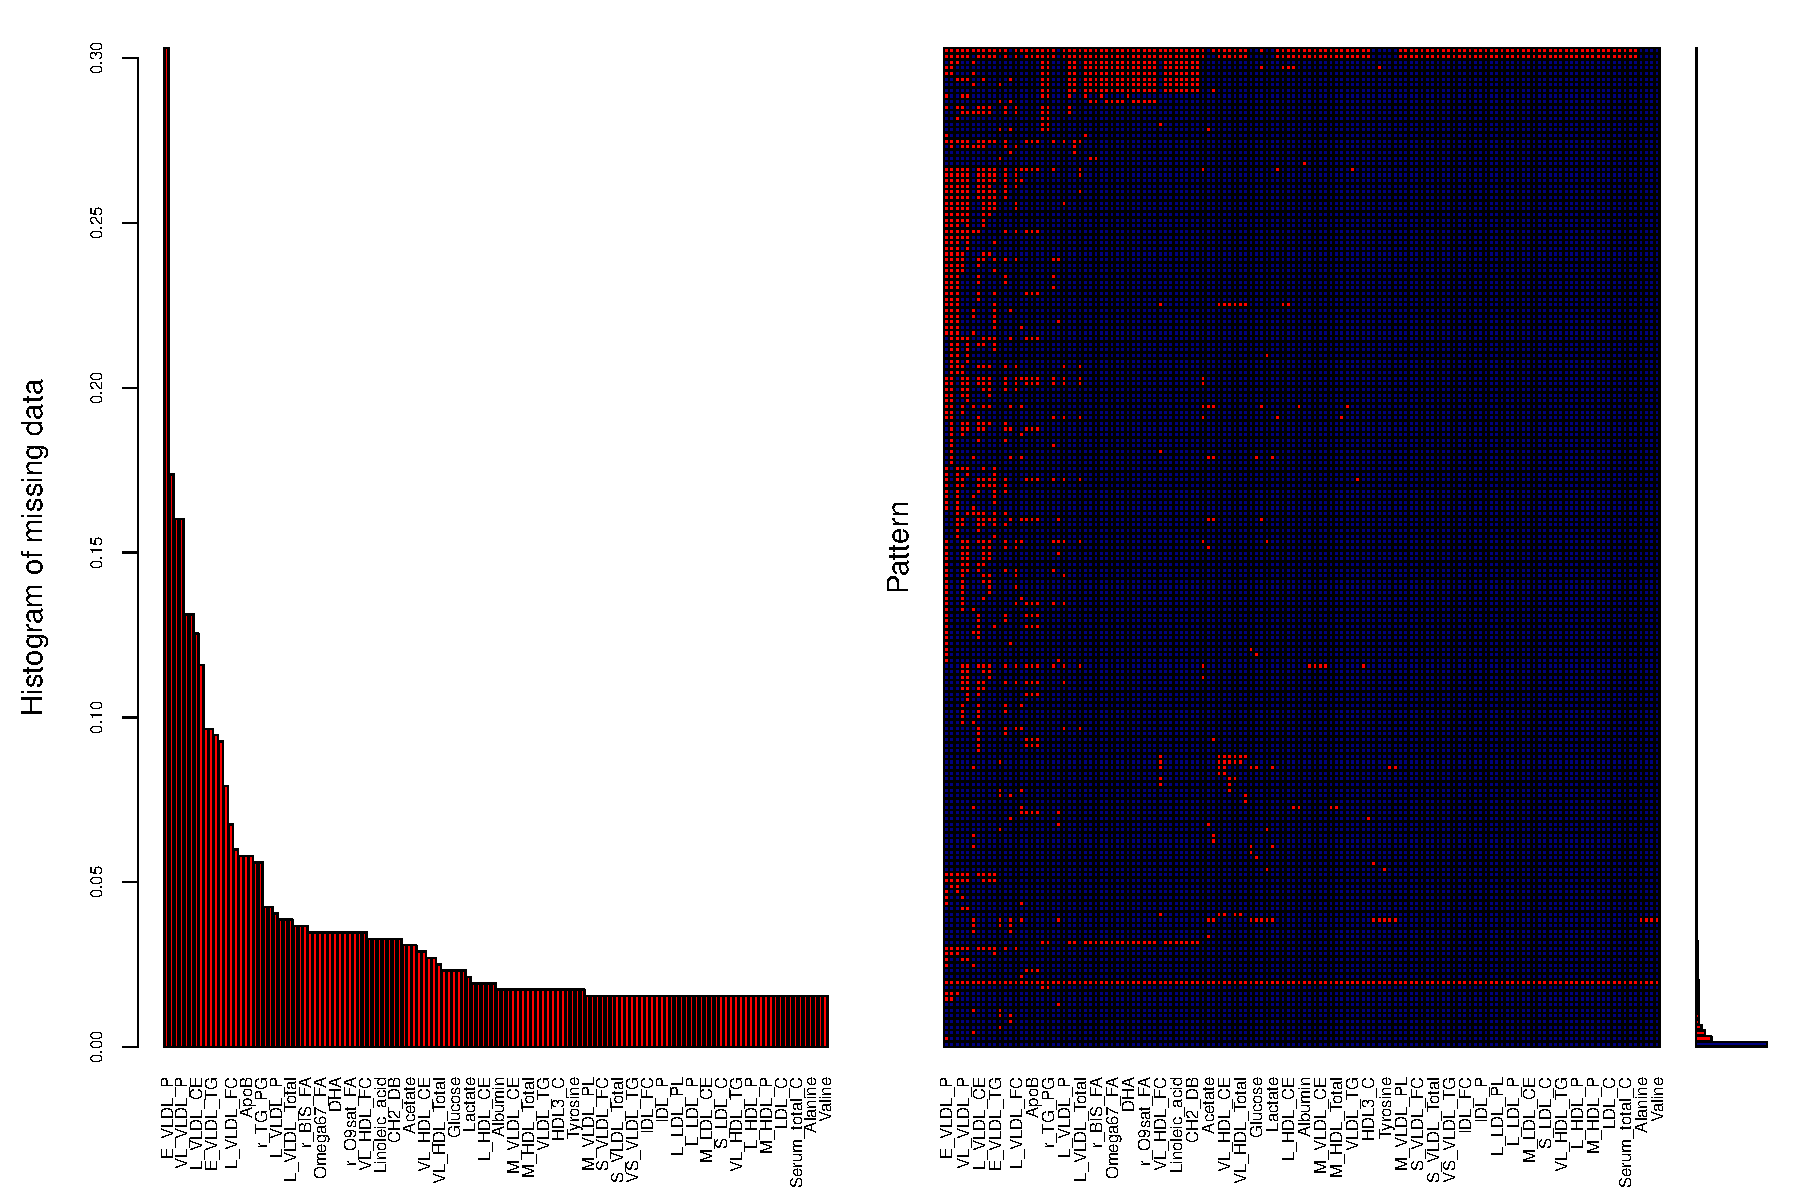
\includegraphics{Figs/Visualize missingness-1.pdf}

\begin{verbatim}
## 
##  Variables sorted by number of missings: 
##           Variable      Count
##           E_VLDL_P 0.30308880
##          E_VLDL_PL 0.17374517
##       E_VLDL_Total 0.16023166
##          VL_VLDL_P 0.16023166
##         VL_VLDL_PL 0.13127413
##           Creatine 0.13127413
##          L_VLDL_CE 0.12548263
##      VL_VLDL_Total 0.11583012
##         VL_VLDL_TG 0.09652510
##          E_VLDL_TG 0.09652510
##       Acetoacetate 0.09459459
##           L_VLDL_C 0.09266409
##  a3hydroxybutyrate 0.07915058
##          L_VLDL_FC 0.06756757
##         Isoleucine 0.05984556
##              ApoAI 0.05791506
##               ApoB 0.05791506
##         ApoB_ApoAI 0.05791506
##           Total_PG 0.05598456
##            r_TG_PG 0.05598456
##          L_VLDL_PL 0.04247104
##                 GP 0.04247104
##           L_VLDL_P 0.04054054
##           Total_TG 0.03861004
##                 SM 0.03861004
##       L_VLDL_Total 0.03861004
##                 PC 0.03667954
##              DB_FA 0.03667954
##           r_BIS_FA 0.03667954
##             Free_C 0.03474903
##          Omega3_FA 0.03474903
##         Omega67_FA 0.03474903
##      Omega9_sat_FA 0.03474903
##           Total_FA 0.03474903
##                DHA 0.03474903
##            r_O3_FA 0.03474903
##           r_O67_FA 0.03474903
##         r_O9sat_FA 0.03474903
##             CH2_FA 0.03474903
##            Avg_FAL 0.03474903
##          VL_HDL_FC 0.03474903
##            Total_C 0.03281853
##       Esterified_C 0.03281853
##      Linoleic_acid 0.03281853
##         Other_PUFA 0.03281853
##     Total_cholines 0.03281853
##             CH2_DB 0.03281853
##           r_BIS_DB 0.03281853
##          L_VLDL_TG 0.03088803
##            Acetate 0.03088803
##            Citrate 0.03088803
##           VL_HDL_C 0.02895753
##          VL_HDL_CE 0.02895753
##          VL_HDL_PL 0.02702703
##           VL_HDL_P 0.02702703
##       VL_HDL_Total 0.02509653
##           L_HDL_FC 0.02316602
##         Creatinine 0.02316602
##            Glucose 0.02316602
##          Glutamine 0.02316602
##      Phenylalanine 0.02316602
##            Lactate 0.02123552
##          M_VLDL_TG 0.01930502
##            L_HDL_C 0.01930502
##           L_HDL_CE 0.01930502
##           M_HDL_CE 0.01930502
##            S_HDL_P 0.01930502
##            Albumin 0.01737452
##           M_VLDL_C 0.01737452
##          M_VLDL_FC 0.01737452
##          M_VLDL_CE 0.01737452
##           S_VLDL_C 0.01737452
##            M_HDL_C 0.01737452
##        M_HDL_Total 0.01737452
##           S_HDL_TG 0.01737452
##        S_HDL_Total 0.01737452
##            VLDL_TG 0.01737452
##     VLDL_TG_lipido 0.01737452
##       IDL_C_lipido 0.01737452
##             HDL3_C 0.01737452
##          Histidine 0.01737452
##            Leucine 0.01737452
##           Tyrosine 0.01737452
##  Unsaturatedlipids 0.01737452
##               Urea 0.01737452
##          M_VLDL_PL 0.01544402
##       M_VLDL_Total 0.01544402
##           M_VLDL_P 0.01544402
##          S_VLDL_FC 0.01544402
##          S_VLDL_PL 0.01544402
##          S_VLDL_TG 0.01544402
##       S_VLDL_Total 0.01544402
##           S_VLDL_P 0.01544402
##         VS_VLDL_PL 0.01544402
##         VS_VLDL_TG 0.01544402
##      VS_VLDL_Total 0.01544402
##          VS_VLDL_P 0.01544402
##             IDL_FC 0.01544402
##             IDL_PL 0.01544402
##          IDL_Total 0.01544402
##              IDL_P 0.01544402
##            L_LDL_C 0.01544402
##           L_LDL_FC 0.01544402
##           L_LDL_PL 0.01544402
##           L_LDL_CE 0.01544402
##        L_LDL_Total 0.01544402
##            L_LDL_P 0.01544402
##            M_LDL_C 0.01544402
##           M_LDL_PL 0.01544402
##           M_LDL_CE 0.01544402
##        M_LDL_Total 0.01544402
##            M_LDL_P 0.01544402
##            S_LDL_C 0.01544402
##        S_LDL_Total 0.01544402
##            S_LDL_P 0.01544402
##          VL_HDL_TG 0.01544402
##           L_HDL_PL 0.01544402
##        L_HDL_Total 0.01544402
##            L_HDL_P 0.01544402
##           M_HDL_FC 0.01544402
##           M_HDL_PL 0.01544402
##            M_HDL_P 0.01544402
##             IDL_TG 0.01544402
##              IDL_C 0.01544402
##              LDL_C 0.01544402
##              HDL_C 0.01544402
##     Serum_total_TG 0.01544402
##      Serum_total_C 0.01544402
##       LDL_C_lipido 0.01544402
##             HDL2_C 0.01544402
##            Alanine 0.01544402
##                CH2 0.01544402
##                CH3 0.01544402
##             Valine 0.01544402
\end{verbatim}

We remove participants with 100\% missing metabolite measurements,
i.e.~missing rows.

\begin{Shaded}
\begin{Highlighting}[]
\NormalTok{NAs_in_metab1 <-}\StringTok{ }\KeywordTok{which}\NormalTok{(}\KeywordTok{apply}\NormalTok{(metab1, }\DecValTok{1}\NormalTok{, function(e) }\KeywordTok{sum}\NormalTok{(}\KeywordTok{is.na}\NormalTok{(e))/}\KeywordTok{length}\NormalTok{(e))==}\DecValTok{1}\NormalTok{)}
\NormalTok{metab2 <-}\StringTok{ }\NormalTok{metab1[-NAs_in_metab1,]}
\NormalTok{rna4 <-}\StringTok{ }\NormalTok{rna3[-NAs_in_metab1,]}
\end{Highlighting}
\end{Shaded}

Random Forests can be used to impute missing metabolites. We use the
\texttt{missForest} package to do this. It takes some time, a couple of
minutes on a modest second generation i5 laptop.

\begin{Shaded}
\begin{Highlighting}[]
\NormalTok{metab2.imp <-}\StringTok{ }\NormalTok{missForest::}\KeywordTok{missForest}\NormalTok{(metab2, }\DataTypeTok{verbose =} \NormalTok{T)}
\end{Highlighting}
\end{Shaded}

\begin{verbatim}
##   missForest iteration 1 in progress...done!
##     estimated error(s): 0.4234906 
##     difference(s): 0.02714137 
##     time: 76.54 seconds
## 
##   missForest iteration 2 in progress...done!
##     estimated error(s): 0.4189017 
##     difference(s): 0.0005727861 
##     time: 75.98 seconds
## 
##   missForest iteration 3 in progress...done!
##     estimated error(s): 0.4185268 
##     difference(s): 0.0002720186 
##     time: 75.55 seconds
## 
##   missForest iteration 4 in progress...done!
##     estimated error(s): 0.4203561 
##     difference(s): 0.0002325965 
##     time: 76.02 seconds
## 
##   missForest iteration 5 in progress...done!
##     estimated error(s): 0.4195952 
##     difference(s): 0.0002338311 
##     time: 75.78 seconds
\end{verbatim}

\begin{Shaded}
\begin{Highlighting}[]
\NormalTok{X2 <-}\StringTok{ }\KeywordTok{scale}\NormalTok{(metab2.imp$ximp, }\DataTypeTok{scale=}\NormalTok{F)}
\NormalTok{X1 <-}\StringTok{ }\KeywordTok{scale}\NormalTok{(rna4, }\DataTypeTok{scale =} \NormalTok{F)}
\end{Highlighting}
\end{Shaded}

In the last two lines, we took one imputed instance of the metabolite
data and centered the columns of the RNA and metabolite data to have
zero mean. We denote them by \texttt{X1} (transcripts) and \texttt{X2}
(metabolites).

\subsubsection{Inspect the data:
descriptives}\label{inspect-the-data-descriptives}

\textbf{Packages needed}

\begin{itemize}
\tightlist
\item
  \texttt{install.packages("gplots")}
\end{itemize}

A heatmap of metabolites, before and after imputation

\begin{Shaded}
\begin{Highlighting}[]
\KeywordTok{try}\NormalTok{(}
  \NormalTok{gplots::}\KeywordTok{heatmap.2}\NormalTok{(}\KeywordTok{cor}\NormalTok{(metab1,}\DataTypeTok{use =} \StringTok{'pair'}\NormalTok{), }\DataTypeTok{Rowv=}\NormalTok{F, }\DataTypeTok{Colv=}\NormalTok{F, }
                    \DataTypeTok{breaks=}\KeywordTok{seq}\NormalTok{(-}\DecValTok{1}\NormalTok{,}\DecValTok{1}\NormalTok{,}\DataTypeTok{length.out =} \DecValTok{25}\NormalTok{), }\DataTypeTok{col=}\NormalTok{gplots::bluered),}
  \DataTypeTok{silent =} \OtherTok{TRUE}\NormalTok{)}
\end{Highlighting}
\end{Shaded}

\begin{verbatim}
## Warning in gplots::heatmap.2(cor(metab1, use = "pair"), Rowv = F, Colv =
## F, : Discrepancy: Rowv is FALSE, while dendrogram is `both'. Omitting row
## dendogram.
\end{verbatim}

\begin{verbatim}
## Warning in gplots::heatmap.2(cor(metab1, use = "pair"), Rowv = F, Colv =
## F, : Discrepancy: Colv is FALSE, while dendrogram is `column'. Omitting
## column dendogram.
\end{verbatim}

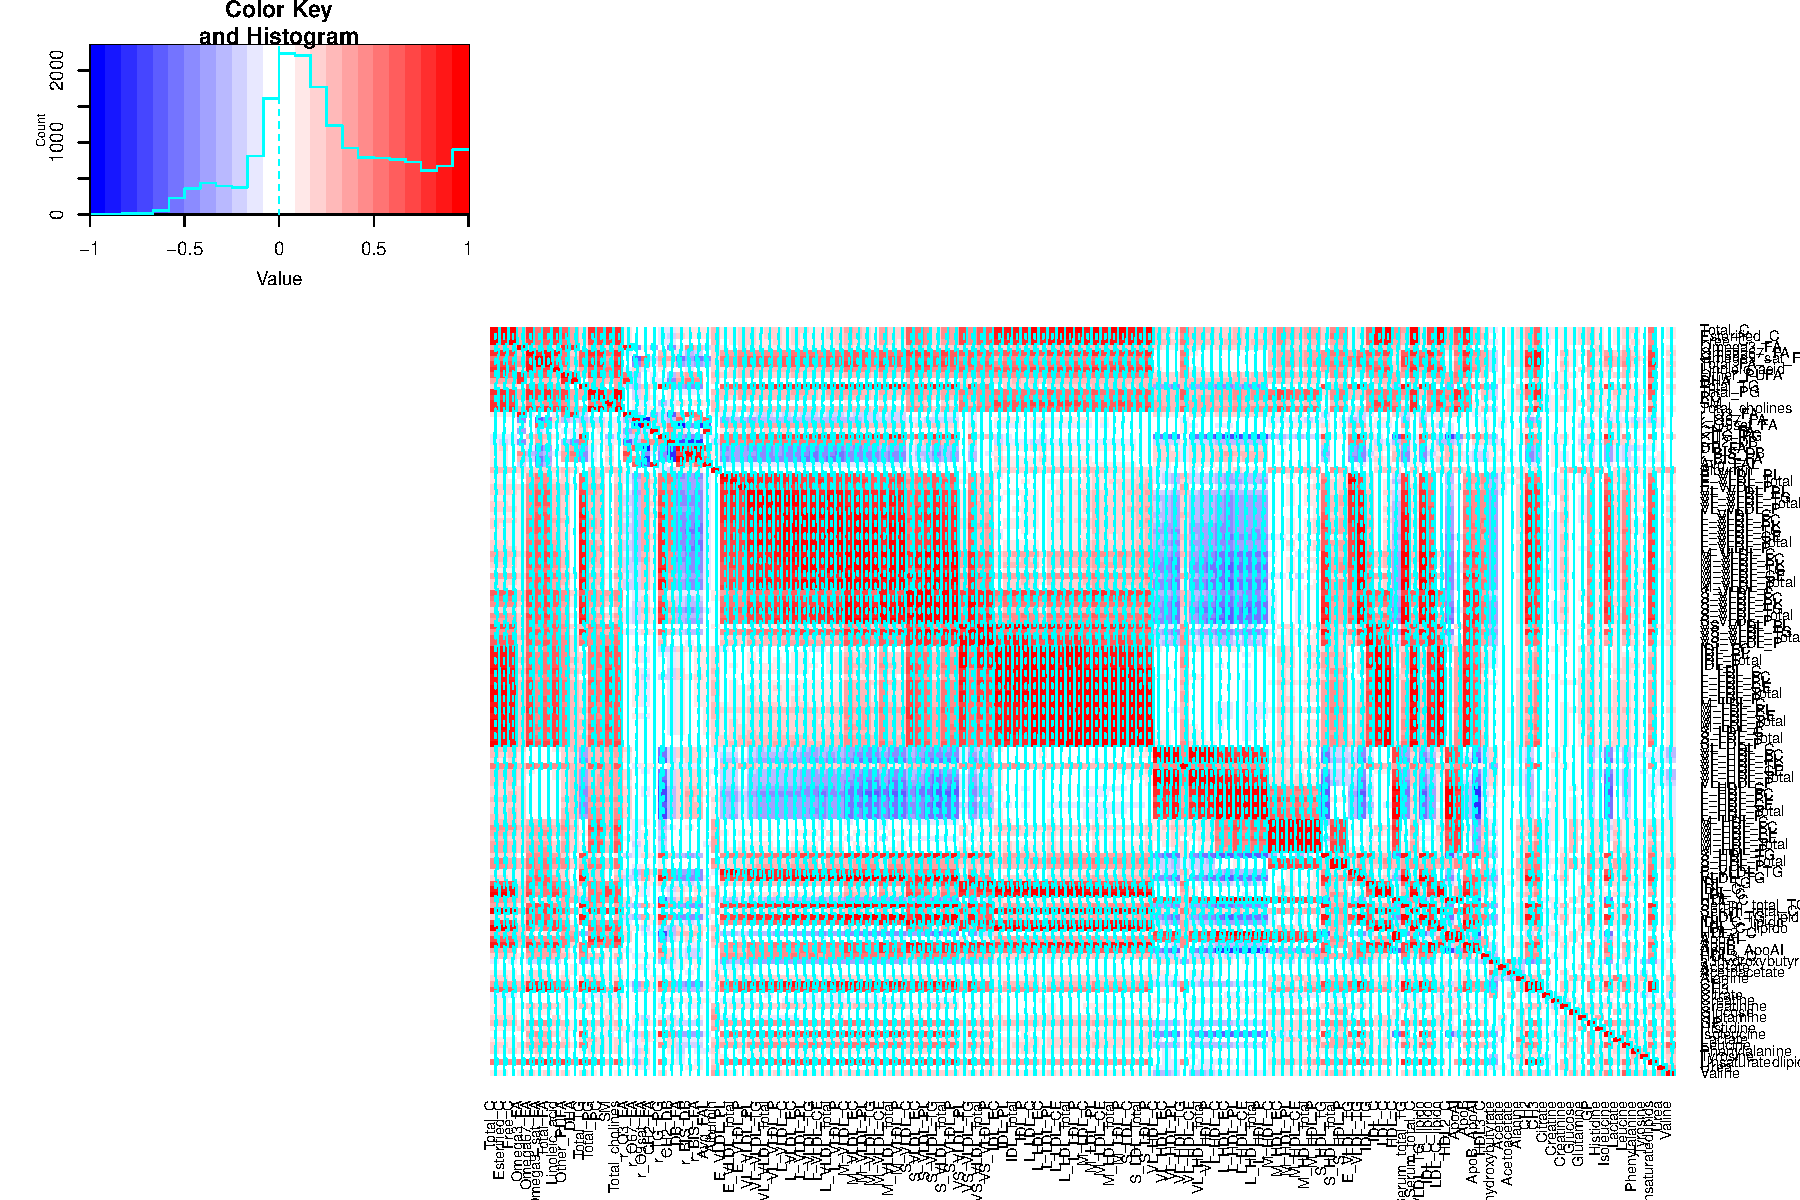
\includegraphics{Figs/Heatmap of correlations-1.pdf}

\begin{Shaded}
\begin{Highlighting}[]
\KeywordTok{try}\NormalTok{(}
  \NormalTok{gplots::}\KeywordTok{heatmap.2}\NormalTok{(}\KeywordTok{cor}\NormalTok{(X2,}\DataTypeTok{use =} \StringTok{'pair'}\NormalTok{), }\DataTypeTok{Rowv=}\NormalTok{F, }\DataTypeTok{Colv=}\NormalTok{F, }
                    \DataTypeTok{breaks=}\KeywordTok{seq}\NormalTok{(-}\DecValTok{1}\NormalTok{,}\DecValTok{1}\NormalTok{,}\DataTypeTok{length.out =} \DecValTok{25}\NormalTok{), }\DataTypeTok{col=}\NormalTok{gplots::bluered),}
  \DataTypeTok{silent =} \OtherTok{TRUE}\NormalTok{)}
\end{Highlighting}
\end{Shaded}

\begin{verbatim}
## Warning in gplots::heatmap.2(cor(X2, use = "pair"), Rowv = F, Colv =
## F, : Discrepancy: Rowv is FALSE, while dendrogram is `both'. Omitting row
## dendogram.
\end{verbatim}

\begin{verbatim}
## Warning in gplots::heatmap.2(cor(X2, use = "pair"), Rowv = F, Colv = F, :
## Discrepancy: Colv is FALSE, while dendrogram is `column'. Omitting column
## dendogram.
\end{verbatim}

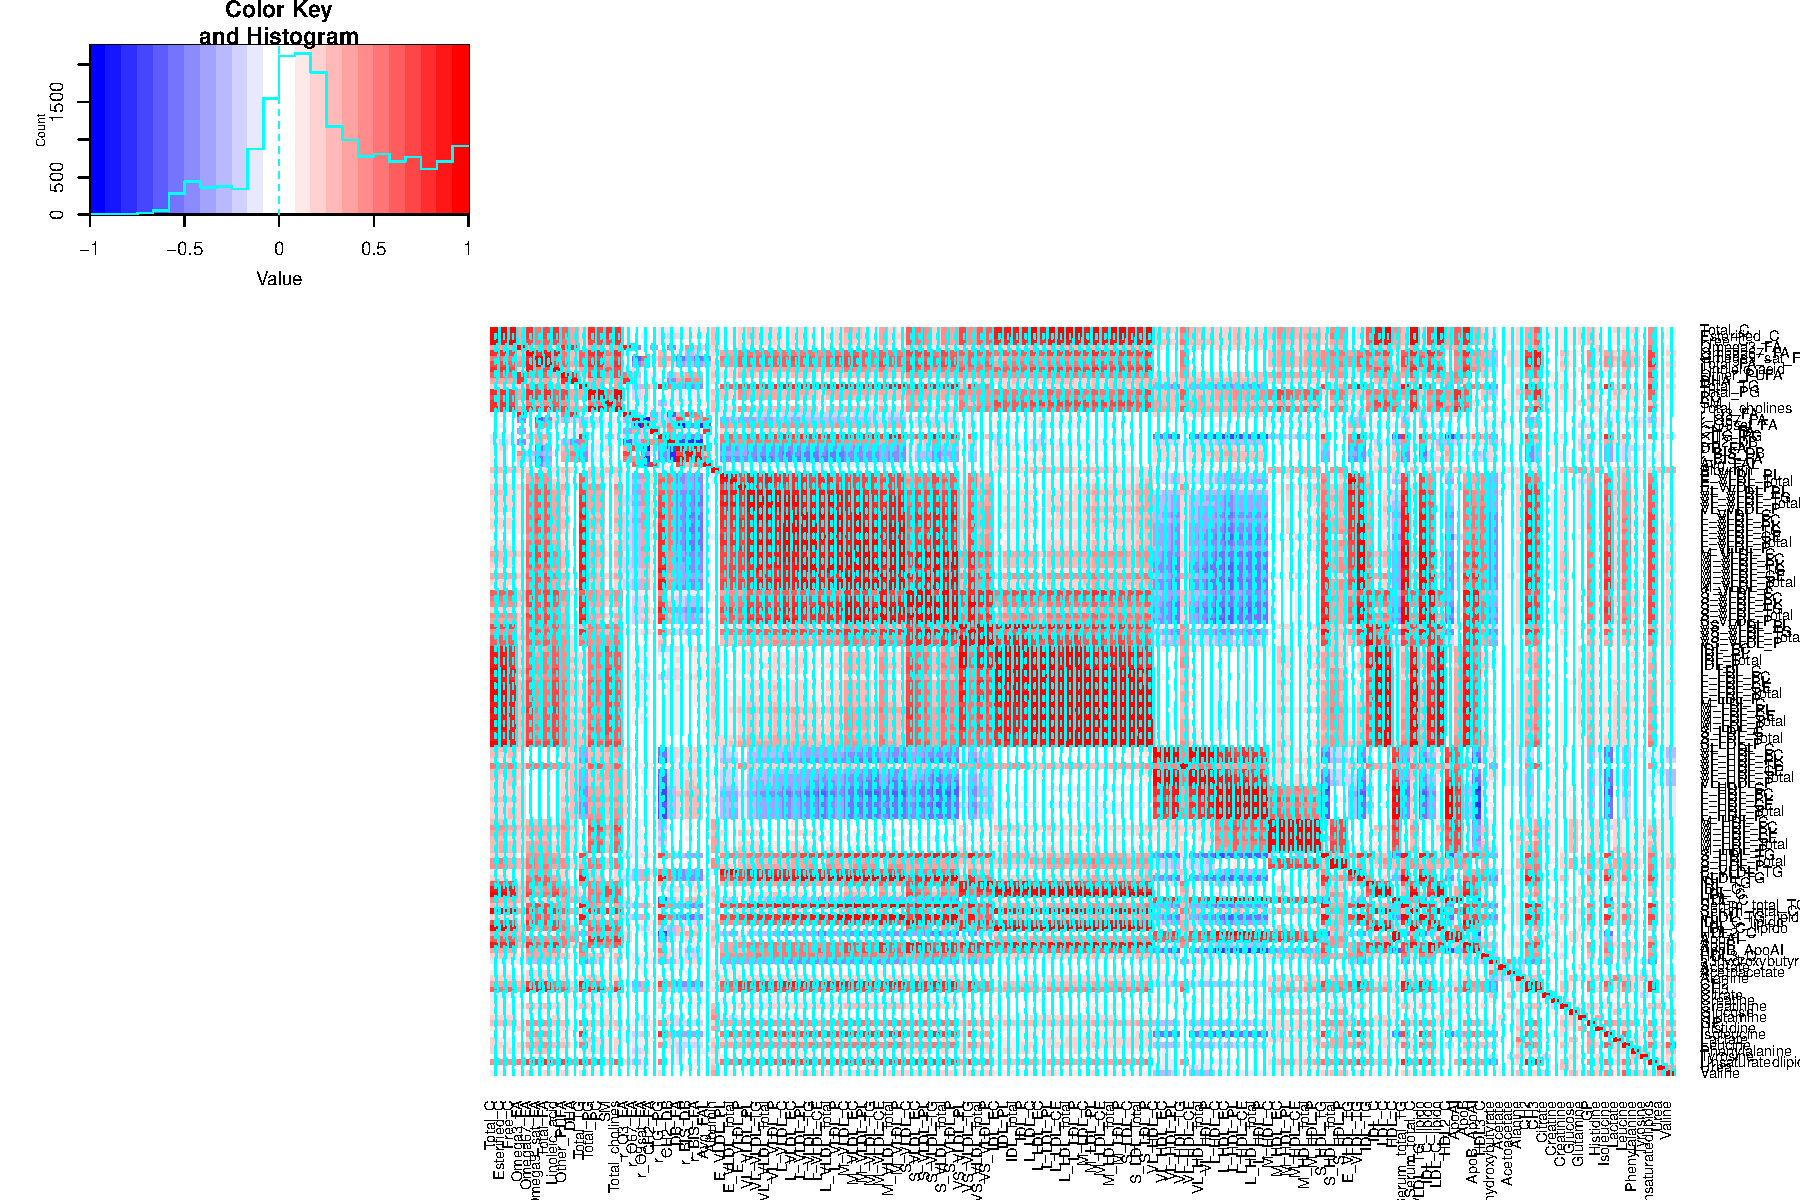
\includegraphics{Figs/Heatmap of correlations-2.pdf} They are almost the
same, indicating that the correlation structure within metabolites
hasn't changed much.

To get an idea on the latent structure of the data one may look at
eigenvalues of covariance matrix of \texttt{X1} and \texttt{X2}.

\begin{Shaded}
\begin{Highlighting}[]
\KeywordTok{svd}\NormalTok{(X1, }\DecValTok{0}\NormalTok{, }\DecValTok{0}\NormalTok{)$d[}\DecValTok{1}\NormalTok{:}\DecValTok{10}\NormalTok{]^}\DecValTok{2} \NormalTok{/}\StringTok{ }\KeywordTok{sum}\NormalTok{(X1^}\DecValTok{2}\NormalTok{)}
\end{Highlighting}
\end{Shaded}

\begin{verbatim}
##  [1] 0.19568455 0.12670559 0.09534211 0.05334638 0.03931151 0.03294359
##  [7] 0.01963035 0.01663232 0.01575400 0.01499442
\end{verbatim}

\begin{Shaded}
\begin{Highlighting}[]
\KeywordTok{svd}\NormalTok{(X2, }\DecValTok{0}\NormalTok{, }\DecValTok{0}\NormalTok{)$d[}\DecValTok{1}\NormalTok{:}\DecValTok{10}\NormalTok{]^}\DecValTok{2} \NormalTok{/}\StringTok{ }\KeywordTok{sum}\NormalTok{(X2^}\DecValTok{2}\NormalTok{)}
\end{Highlighting}
\end{Shaded}

\begin{verbatim}
##  [1] 0.37544553 0.21076846 0.10669151 0.04796332 0.03171004 0.02697083
##  [7] 0.02085717 0.01758810 0.01569650 0.01329923
\end{verbatim}

\begin{Shaded}
\begin{Highlighting}[]
\KeywordTok{svd}\NormalTok{(}\KeywordTok{crossprod}\NormalTok{(X1,X2),}\DecValTok{0}\NormalTok{,}\DecValTok{0}\NormalTok{)$d[}\DecValTok{1}\NormalTok{:}\DecValTok{20}\NormalTok{]}
\end{Highlighting}
\end{Shaded}

\begin{verbatim}
##  [1] 7109.2911 3885.6227 2453.7749 2364.2937 1990.4501 1226.8889 1156.0470
##  [8]  986.7474  780.6249  747.3281  691.4328  616.8352  579.9895  514.3137
## [15]  490.8930  429.8551  410.8972  368.9870  356.8286  346.3882
\end{verbatim}

The first two lines contain relative variances explained by each
principal component. Strong latent structure is indicated by a sharp
decline of the relative variances at the first few components.

Boxplots are a good summary to check the distribution of the variables
relative to each other. Properties such as comparable means, variances
and symmetry are often good to have. To reduce the number of boxplots we
filter the transcriptomic data to include genes with 95\% highest
expression and IQR.

\begin{Shaded}
\begin{Highlighting}[]
\KeywordTok{boxplot}\NormalTok{(X1[,}\KeywordTok{filter_rna}\NormalTok{(X1, .}\DecValTok{95}\NormalTok{)])}
\end{Highlighting}
\end{Shaded}

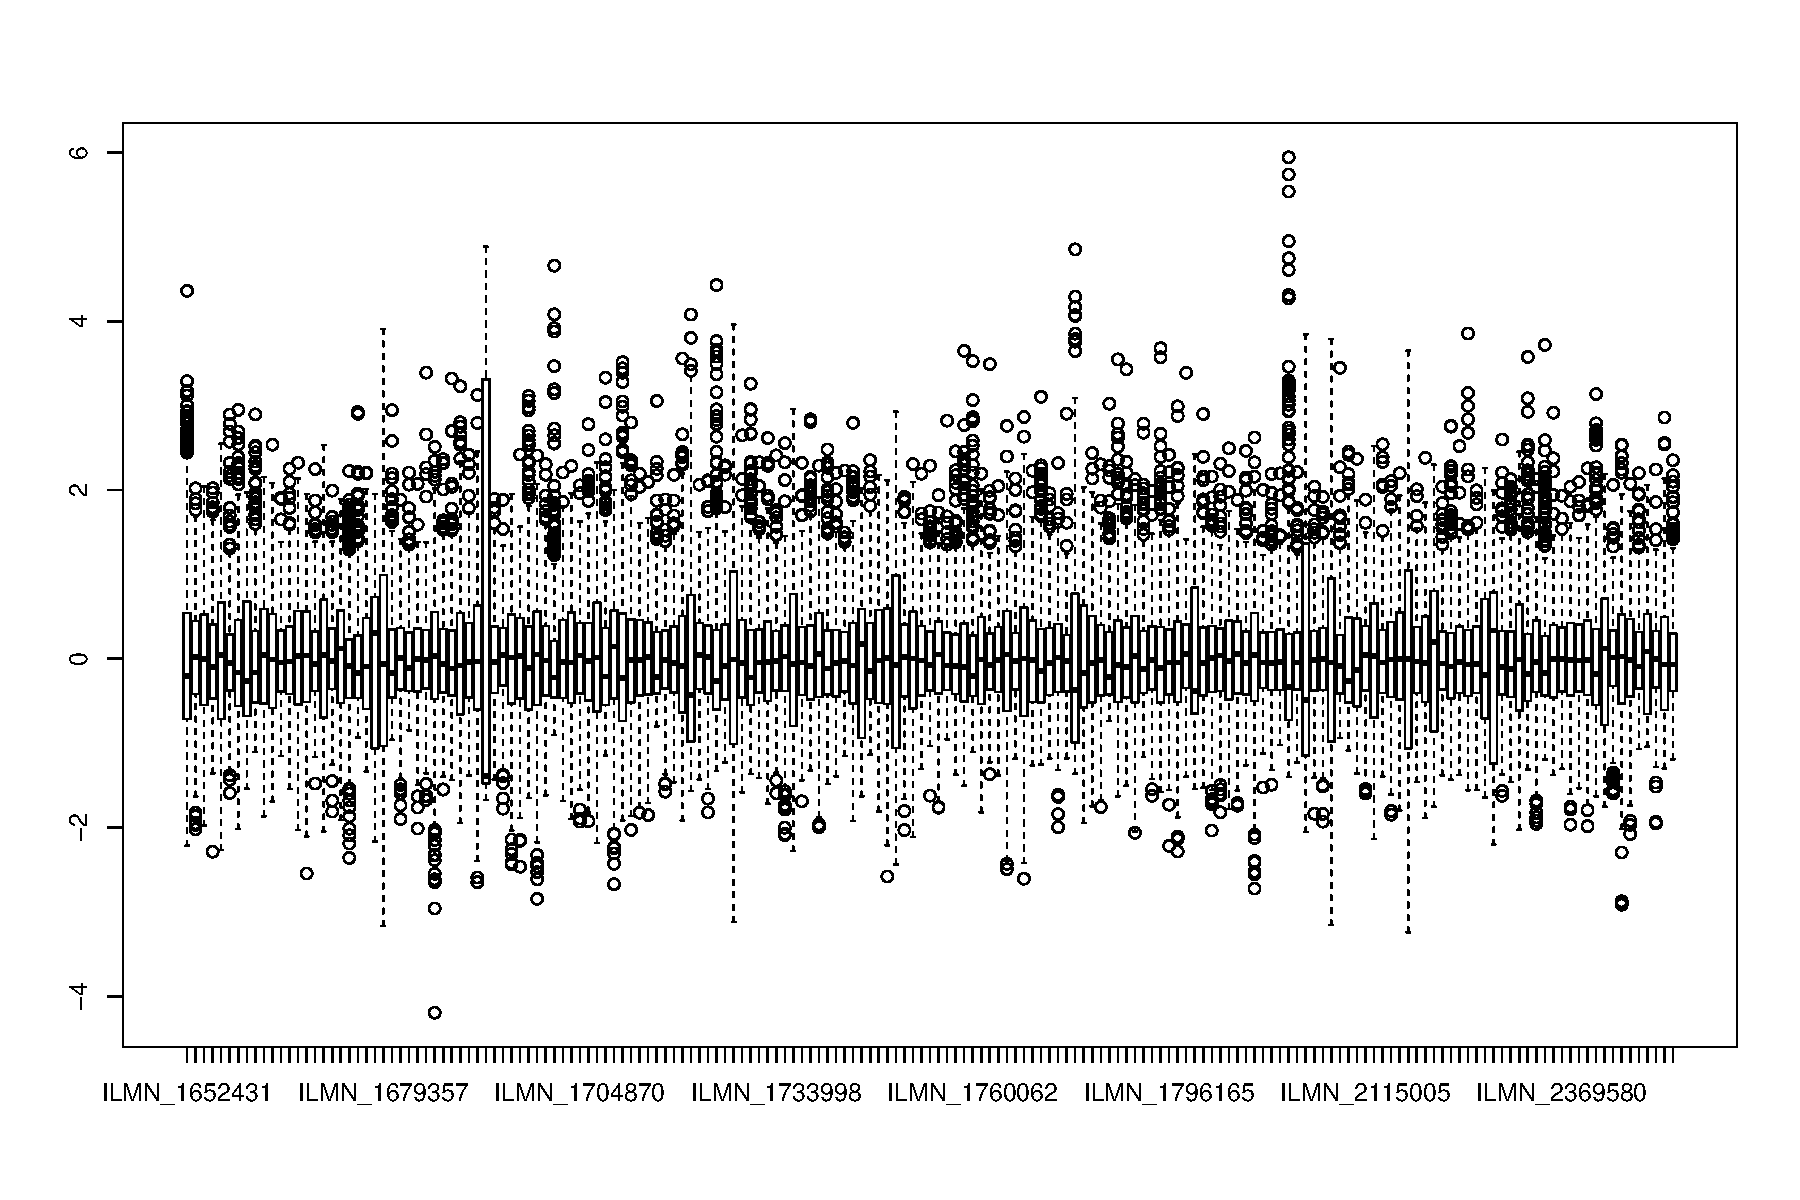
\includegraphics{Figs/Boxplots-1.pdf}

\begin{Shaded}
\begin{Highlighting}[]
\KeywordTok{boxplot}\NormalTok{(X2)}
\end{Highlighting}
\end{Shaded}

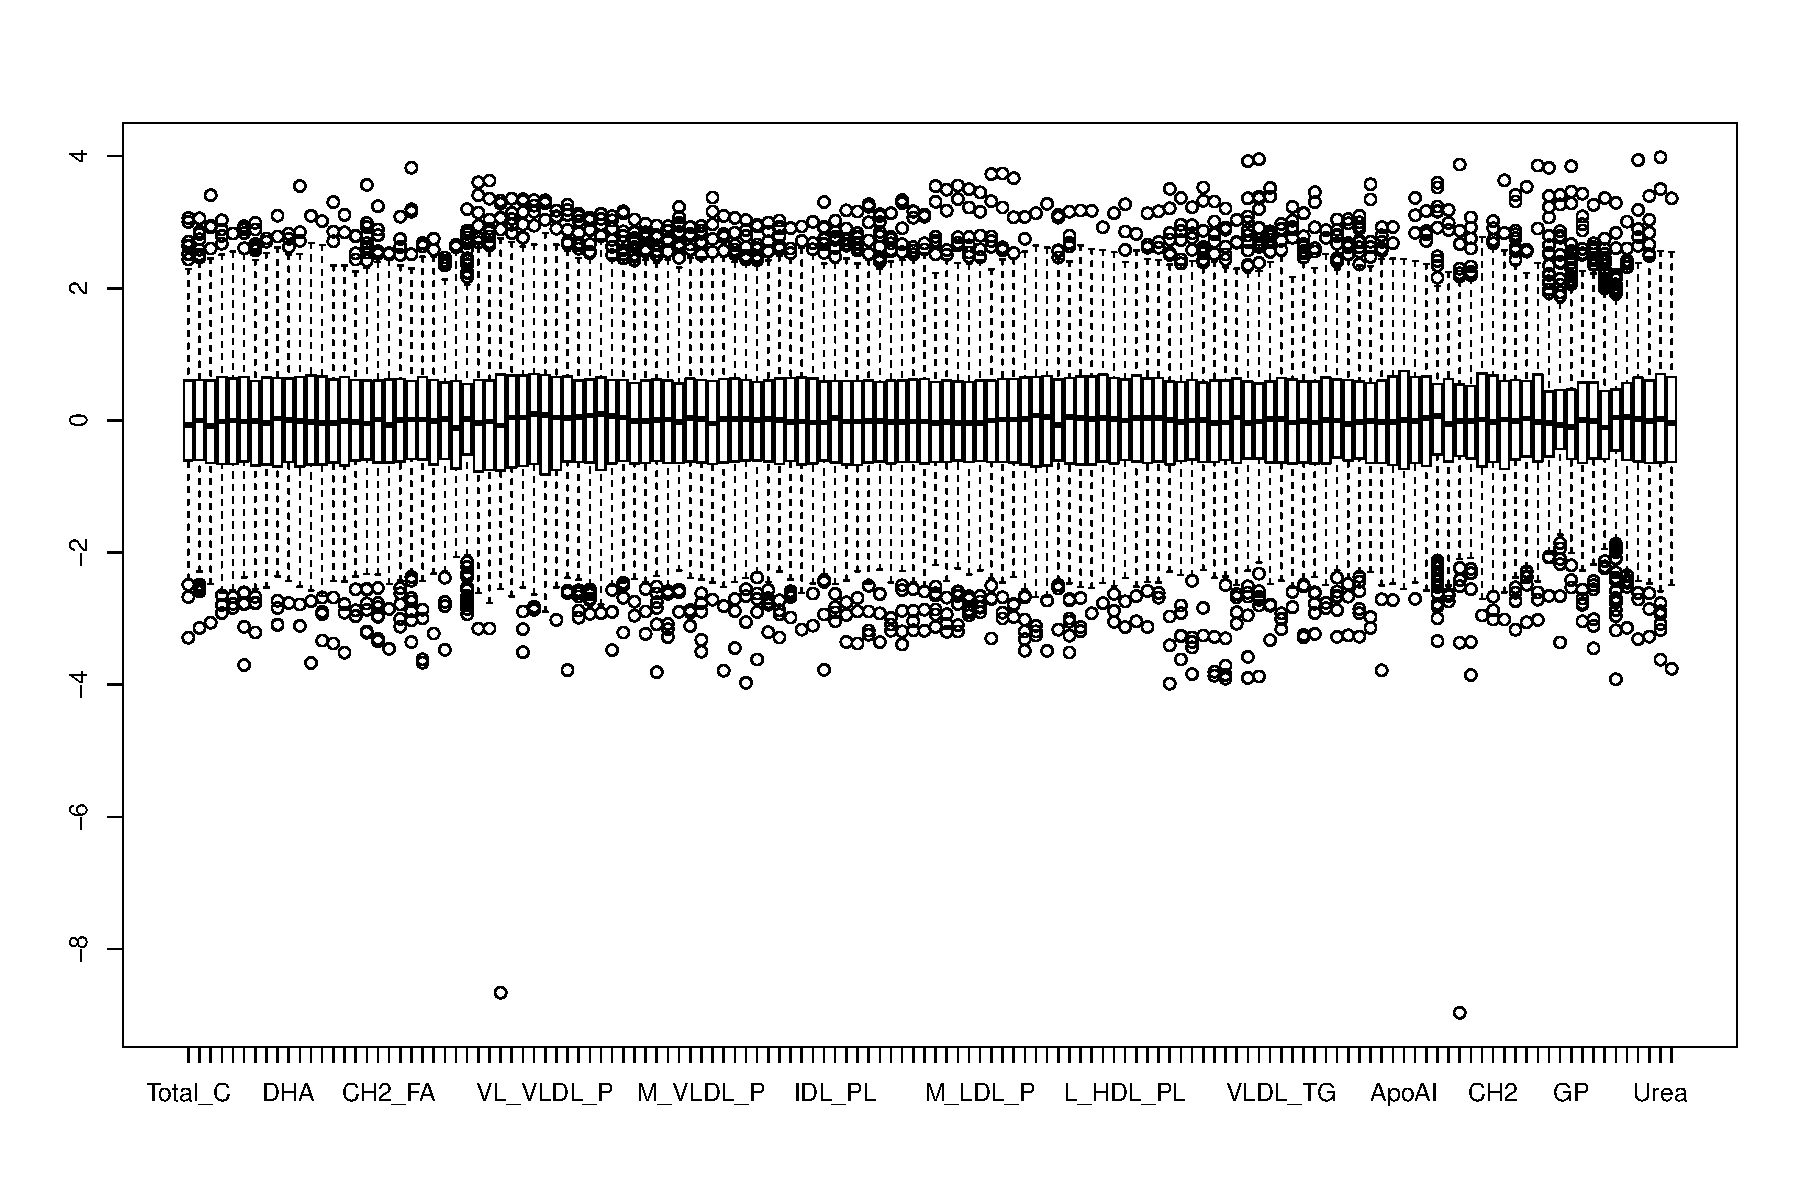
\includegraphics{Figs/Boxplots-2.pdf}

\subsection{The OmicsPLS package}\label{the-omicspls-package}

\subsubsection{Cross-validation}\label{cross-validation-1}

We load the OmicsPLS package and set a seed for the cross-validation.
The strategy is to have a relatively large grid to search on and apply
the faster alternative Cross-Validation (Cv) approach to find a
solution. Then on a smaller grid containing these integers we do a full
CV to determine the best choice for the number of components. The
objective function to minimize is the sum of the two prediction errors
\(||X-\hat{X}||\) and \(||Y-\hat{Y}||\).

\begin{Shaded}
\begin{Highlighting}[]
\KeywordTok{library}\NormalTok{(OmicsPLS)}
\KeywordTok{set.seed}\NormalTok{(}\DecValTok{1+1+2016}\NormalTok{)}
\CommentTok{#CV1 <- crossval_o2m_adjR2(X1, X2, 1:3, c(0,1,5,10), c(0,1,5,10), nr_folds = 2, nr_cores = 4)}
\CommentTok{#CV2 <- crossval_o2m(X1, X2, 1:2, 0:2, 9:11, nr_folds = 10, nr_cores = 4)}
\CommentTok{#CV1}
\CommentTok{#CV2}
\end{Highlighting}
\end{Shaded}

Following the advice of the last CV output, we select two joint, one
transcript-specific and ten metabolite-specific components. We fit the
O2PLS model with default values as follows.

\begin{Shaded}
\begin{Highlighting}[]
\NormalTok{fit =}\StringTok{ }\KeywordTok{o2m}\NormalTok{(X1, X2, }\DecValTok{2}\NormalTok{, }\DecValTok{1}\NormalTok{, }\DecValTok{10}\NormalTok{)}
\NormalTok{fit}
\end{Highlighting}
\end{Shaded}

\begin{verbatim}
## O2PLS fit 
## with 2 joint components  
## and  1 orthogonal components in X 
## and  10 orthogonal components in Y 
## Elapsed time: 3.12 sec
\end{verbatim}

A summary of the variation modeled is obtained via

\begin{Shaded}
\begin{Highlighting}[]
\KeywordTok{summary}\NormalTok{(fit)}
\end{Highlighting}
\end{Shaded}

\begin{verbatim}
## 
## *** Summary of the O2PLS fit *** 
## 
## -  Call: o2m(X = X1, Y = X2, n = 2, nx = 1, ny = 10) 
## 
## -  Modeled variation
## -- Total variation:
## in X: 332035.7 
## in Y: 68381.71 
## 
## -- Joint, Orthogonal and Noise as proportions:
## 
##            data X data Y
## Joint       0.124  0.410
## Orthogonal  0.171  0.243
## Noise       0.705  0.348
## 
## -- Predictable variation in Y-joint part by X-joint part:
## Variation in Yhat relative to U: 0.116 
## -- Predictable variation in X-joint part by Y-joint part:
## Variation in Xhat relative to T: 0.151 
## 
## -- Variances per component:
## 
##           Comp 1    Comp 2
## X joint 25039.63 16203.728
## Y joint 18456.89  9555.336
## 
##          Comp 1
## X Orth 56637.85
## 
##          Comp 1   Comp 2   Comp 3   Comp 4   Comp 5   Comp 6  Comp 7
## Y Orth 6715.068 3315.059 2055.242 1199.923 1091.131 1103.341 838.014
##         Comp 8  Comp 9 Comp 10
## Y Orth 950.716 570.621 850.223
## 
## 
## -  Coefficient in 'U = T B_T + H_U' model:
## -- Diagonal elements of B_T =
##  0.401 0.339
\end{verbatim}

\subsubsection{Plotting}\label{plotting}

\textbf{Packages needed}

\begin{itemize}
\tightlist
\item
  \texttt{install.packages("magrittr")}
\item
  \texttt{install.packages("ggplot2")}
\item
  \texttt{install.packages("gridExtra")}
\item
  \texttt{install.packages("stringr")}
\item
  \texttt{install.packages("gplots")}
\end{itemize}

We want to see which (groups of) metabolites and transcripts tend to
correlate with each other. To do this we plot the loadings. The
individual loading values per component indicate the relative importance
of each variable to the corresponding component. We plot the two joint
loadings against each other to see which metabolites are more important
for each component. To do this we need three packages for convenience:
\texttt{magrittr} for the piping operator, \texttt{ggplot2} for plotting
and \texttt{gridExtra} to put multiple ggplots in one figure. Also
\texttt{stringr} will be needed to extract substrings of column names.

\begin{Shaded}
\begin{Highlighting}[]
\KeywordTok{require}\NormalTok{(magrittr)}
\end{Highlighting}
\end{Shaded}

\begin{verbatim}
## Loading required package: magrittr
\end{verbatim}

\begin{Shaded}
\begin{Highlighting}[]
\KeywordTok{require}\NormalTok{(ggplot2)}
\end{Highlighting}
\end{Shaded}

\begin{verbatim}
## Loading required package: ggplot2
\end{verbatim}

\begin{Shaded}
\begin{Highlighting}[]
\KeywordTok{require}\NormalTok{(gridExtra)}
\end{Highlighting}
\end{Shaded}

\begin{verbatim}
## Loading required package: gridExtra
\end{verbatim}

\begin{Shaded}
\begin{Highlighting}[]
\CommentTok{# Color names}
\NormalTok{name_col =}\StringTok{ }\DecValTok{1} \NormalTok{+}\StringTok{ }\KeywordTok{sapply}\NormalTok{( }\CommentTok{#First sapply loops over column names}
  \DataTypeTok{X =} \KeywordTok{colnames}\NormalTok{(X2),}
  \DataTypeTok{FUN =} \NormalTok{function(arg)\{}
    \KeywordTok{crossprod}\NormalTok{(}
      \KeywordTok{c}\NormalTok{(}\DecValTok{1}\NormalTok{, }\DecValTok{1}\NormalTok{, }\DecValTok{3}\NormalTok{), }\CommentTok{# Weights to be used as categories}
      \KeywordTok{sapply}\NormalTok{(}\KeywordTok{c}\NormalTok{(}\StringTok{"VLDL"}\NormalTok{, }\StringTok{"LDL"}\NormalTok{, }\StringTok{"HDL"}\NormalTok{), }\CommentTok{# metabolite classes}
             \NormalTok{function(arg2)\{}\KeywordTok{grepl}\NormalTok{(arg2, arg)\} }\CommentTok{# compare class of metabolites}
      \NormalTok{)}
    \NormalTok{)}
    \NormalTok{\}}
  \NormalTok{)}

\NormalTok{alpX2 <-}\StringTok{ }\KeywordTok{loadings}\NormalTok{(fit, }\StringTok{"Yjoint"}\NormalTok{, }\DecValTok{1}\NormalTok{:}\DecValTok{2}\NormalTok{) %>%}\StringTok{  }\CommentTok{# Retreive loadings}
\StringTok{  }\NormalTok{abs %>%}\StringTok{ }\CommentTok{# Absolute loading values for positive weights}
\StringTok{  }\NormalTok{rowSums %>%}\StringTok{ }\CommentTok{# Sum over the components}
\StringTok{  }\NormalTok{sqrt +}\StringTok{ }\NormalTok{(name_col>}\DecValTok{1}\NormalTok{) }\CommentTok{# Take square root}

\NormalTok{######### Plot loadings with OmicsPLS plot method ###}
\NormalTok{p_X2 <-}\StringTok{ }\KeywordTok{plot}\NormalTok{(fit, }\DataTypeTok{loading_name=}\StringTok{"Yj"}\NormalTok{, }\DataTypeTok{i=}\DecValTok{1}\NormalTok{, }\DataTypeTok{j=}\DecValTok{2}\NormalTok{, }\DataTypeTok{label=}\StringTok{"c"}\NormalTok{, }\CommentTok{# Plot the loadings}
             \DataTypeTok{alpha=}\DecValTok{0}\NormalTok{) +}\StringTok{ }\CommentTok{# set points to be 100% transparant}
\NormalTok{##################### Add all layers ###}
\StringTok{  }\KeywordTok{theme_bw}\NormalTok{() +}\StringTok{ }
\StringTok{  }\KeywordTok{coord_fixed}\NormalTok{(}\DataTypeTok{ratio =} \DecValTok{1}\NormalTok{, }\DataTypeTok{xlim=}\KeywordTok{c}\NormalTok{(-.}\DecValTok{2}\NormalTok{,.}\DecValTok{2}\NormalTok{),}\DataTypeTok{ylim=}\KeywordTok{c}\NormalTok{(-.}\DecValTok{2}\NormalTok{,.}\DecValTok{2}\NormalTok{)) +}
\StringTok{  }\KeywordTok{geom_point}\NormalTok{( }\CommentTok{# Set color and size}
    \KeywordTok{aes}\NormalTok{(}\DataTypeTok{col=}\KeywordTok{factor}\NormalTok{(name_col, }\DataTypeTok{levels =} \DecValTok{4}\NormalTok{:}\DecValTok{1}\NormalTok{), }\DataTypeTok{size =} \KeywordTok{I}\NormalTok{(}\DecValTok{1}\NormalTok{+(name_col>}\DecValTok{1}\NormalTok{)), }\DataTypeTok{shape =} 
          \KeywordTok{factor}\NormalTok{(name_col, }\DataTypeTok{levels =} \DecValTok{4}\NormalTok{:}\DecValTok{1}\NormalTok{)),}\DataTypeTok{show.legend =} \NormalTok{T) +}
\StringTok{  }\KeywordTok{theme}\NormalTok{(}\DataTypeTok{legend.position=}\StringTok{"right"}\NormalTok{) +}\StringTok{ }
\StringTok{  }\KeywordTok{scale_color_discrete}\NormalTok{(}\DataTypeTok{name=}\StringTok{"Metabolite}\CharTok{\textbackslash{}n}\StringTok{Group"}\NormalTok{, }
                       \DataTypeTok{labels=}\KeywordTok{c}\NormalTok{(}\StringTok{"LDL"}\NormalTok{,}\StringTok{"VLDL"}\NormalTok{,}\StringTok{"HDL"}\NormalTok{,}\StringTok{"Other"}\NormalTok{)) +}
\StringTok{  }\KeywordTok{guides}\NormalTok{(}\DataTypeTok{size=}\NormalTok{F) +}\StringTok{ }\KeywordTok{scale_shape_discrete}\NormalTok{(}\DataTypeTok{name=}\StringTok{"Metabolite}\CharTok{\textbackslash{}n}\StringTok{Group"}\NormalTok{, }
                                        \DataTypeTok{labels=}\KeywordTok{c}\NormalTok{(}\StringTok{"LDL"}\NormalTok{,}\StringTok{"VLDL"}\NormalTok{,}\StringTok{"HDL"}\NormalTok{,}\StringTok{"Other"}\NormalTok{)) +}
\KeywordTok{labs}\NormalTok{(}\DataTypeTok{title =} \StringTok{"Metabolite joint loadings"}\NormalTok{, }
     \DataTypeTok{x =} \StringTok{"First Joint Loadings"}\NormalTok{, }\DataTypeTok{y =} \StringTok{"Second Joint Loadings"}\NormalTok{) +}
\StringTok{  }\KeywordTok{theme}\NormalTok{(}\DataTypeTok{plot.title =} \KeywordTok{element_text}\NormalTok{(}\DataTypeTok{face=}\StringTok{'bold'}\NormalTok{), }
        \DataTypeTok{legend.title=}\KeywordTok{element_text}\NormalTok{(}\DataTypeTok{face=}\StringTok{'bold'}\NormalTok{)) }

\NormalTok{alpX1 <-}\StringTok{ }\KeywordTok{loadings}\NormalTok{(fit, }\StringTok{"Xjoint"}\NormalTok{, }\DecValTok{1}\NormalTok{:}\DecValTok{2}\NormalTok{) %>%}\StringTok{ }\KeywordTok{raise_to_power}\NormalTok{(}\DecValTok{2}\NormalTok{) %>%}\StringTok{ }\NormalTok{rowSums}
\NormalTok{alpX1[-(}\KeywordTok{order}\NormalTok{(alpX1,}\DataTypeTok{decreasing=}\NormalTok{T)[}\DecValTok{1}\NormalTok{:}\DecValTok{10}\NormalTok{])] =}\StringTok{ }\DecValTok{0}
\NormalTok{alpX1 <-}\StringTok{ }\KeywordTok{sign}\NormalTok{(alpX1)}
\NormalTok{######### Plot loadings with OmicsPLS plot method ###}
\NormalTok{p_X1 <-}\StringTok{ }\KeywordTok{plot}\NormalTok{(fit, }\DataTypeTok{loading_name=}\StringTok{"Xj"}\NormalTok{, }\DataTypeTok{i=}\DecValTok{1}\NormalTok{, }\DataTypeTok{j=}\DecValTok{2}\NormalTok{, }\DataTypeTok{label =} \StringTok{"c"}\NormalTok{, }\DataTypeTok{use_ggplot2 =} \OtherTok{TRUE}\NormalTok{,}
             \DataTypeTok{alpha =} \NormalTok{alpX1, }
             \KeywordTok{aes}\NormalTok{(}\DataTypeTok{label =} \NormalTok{stringr::}\KeywordTok{str_sub}\NormalTok{(}\KeywordTok{colnames}\NormalTok{(X1), }\DataTypeTok{start =} \DecValTok{6}\NormalTok{)),}
             \DataTypeTok{hjust =} \KeywordTok{rep}\NormalTok{(}\KeywordTok{c}\NormalTok{(}\DecValTok{0}\NormalTok{, }\DecValTok{1}\NormalTok{), }\DataTypeTok{length.out =} \KeywordTok{ncol}\NormalTok{(X1))) +}\StringTok{ }
\NormalTok{##################### Add all layers ###}
\StringTok{  }\KeywordTok{theme_bw}\NormalTok{() +}\StringTok{ }
\StringTok{  }\KeywordTok{coord_fixed}\NormalTok{(.}\DecValTok{8}\NormalTok{, }\KeywordTok{c}\NormalTok{(-.}\DecValTok{15}\NormalTok{,.}\DecValTok{15}\NormalTok{),}\KeywordTok{c}\NormalTok{(-.}\DecValTok{15}\NormalTok{,.}\DecValTok{15}\NormalTok{)) +}
\StringTok{  }\KeywordTok{geom_point}\NormalTok{(}\DataTypeTok{alpha =} \FloatTok{0.5+0.5}\NormalTok{*alpX1, }\DataTypeTok{col =} \StringTok{'grey'}\NormalTok{) +}\StringTok{ }
\StringTok{  }\KeywordTok{labs}\NormalTok{(}\DataTypeTok{title =} \StringTok{"Transcript joint loadings"}\NormalTok{, }
       \DataTypeTok{x =} \StringTok{"First Joint Loadings"}\NormalTok{, }\DataTypeTok{y =} \StringTok{"Second Joint Loadings"}\NormalTok{) +}
\StringTok{  }\KeywordTok{theme}\NormalTok{(}\DataTypeTok{plot.title =} \KeywordTok{element_text}\NormalTok{(}\DataTypeTok{face=}\StringTok{'bold'}\NormalTok{))}

\NormalTok{## Finally plot both plots in one figure.}
\KeywordTok{grid.arrange}\NormalTok{(p_X2, p_X1, }\DataTypeTok{ncol=}\DecValTok{2}\NormalTok{)}
\end{Highlighting}
\end{Shaded}

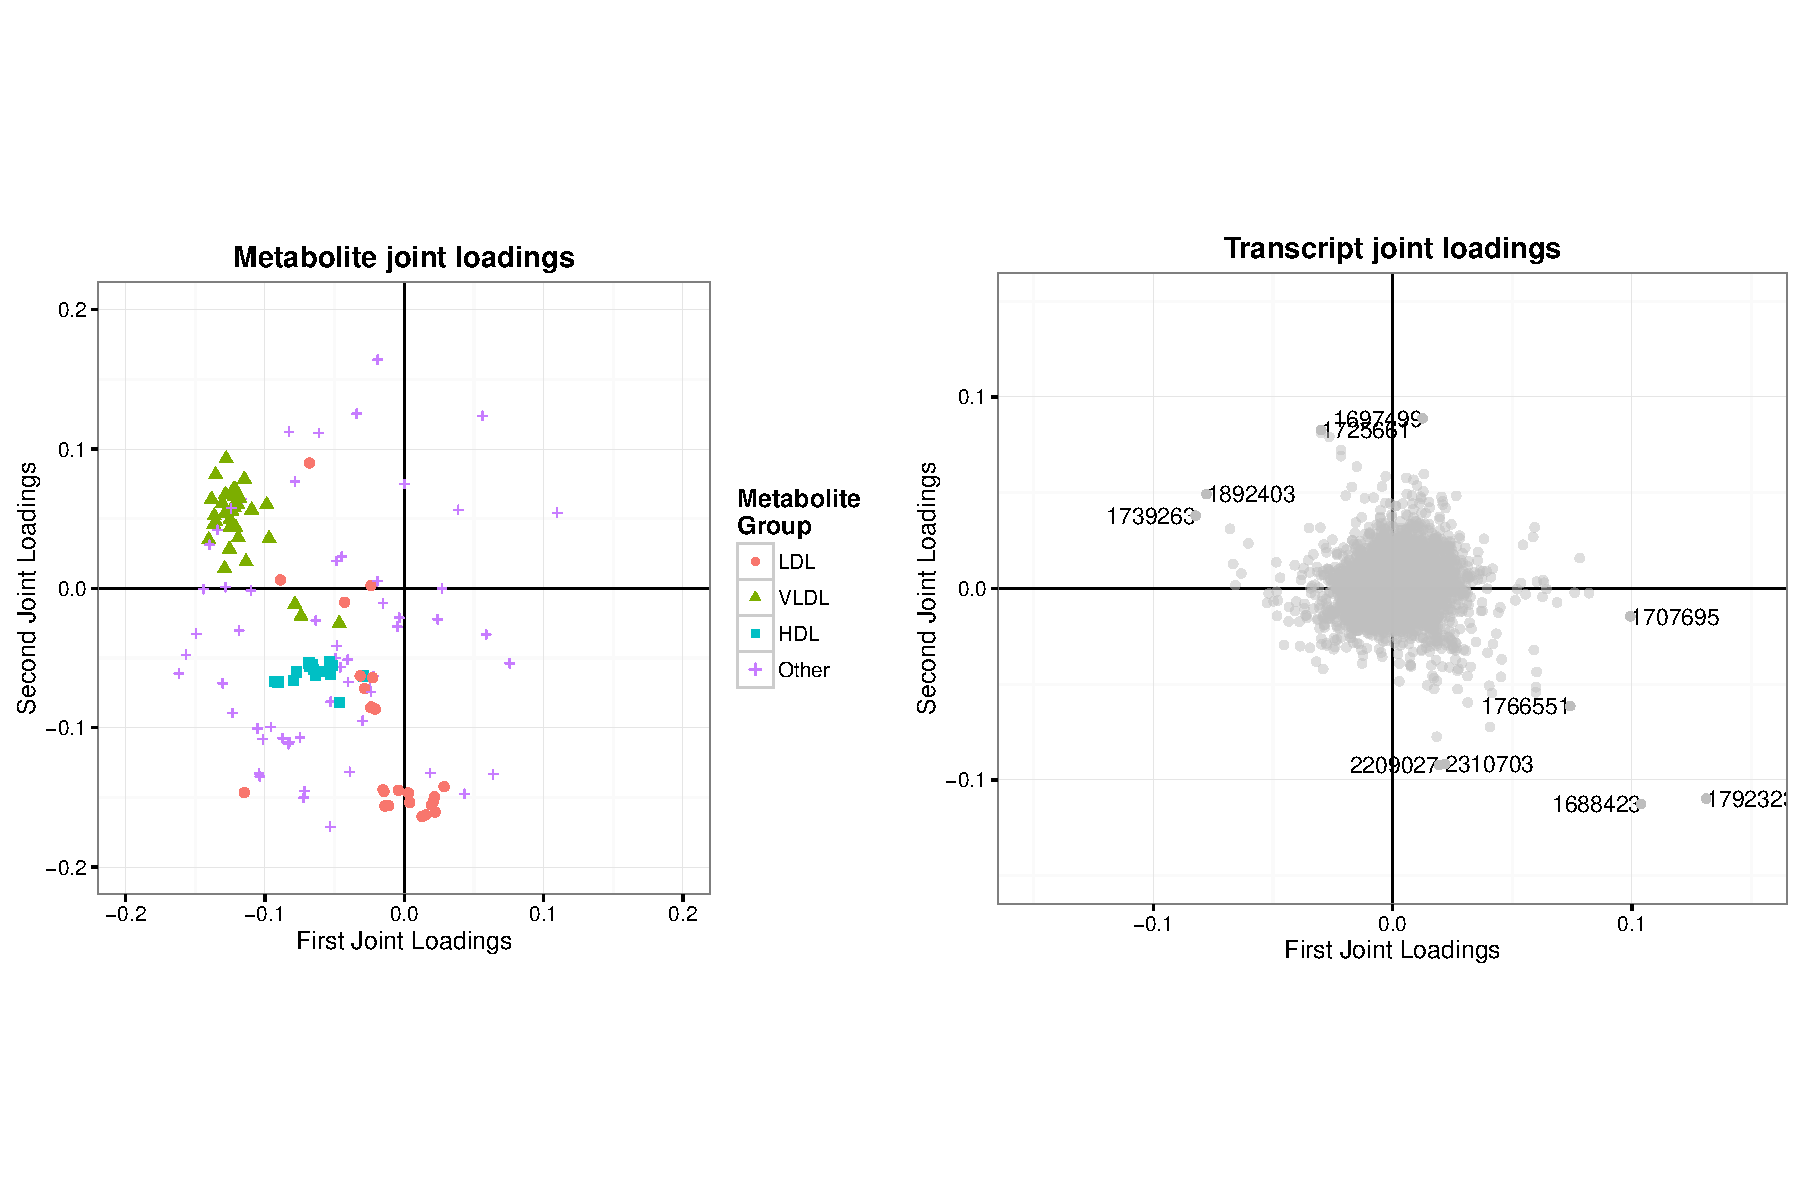
\includegraphics{Figs/Loadings plot-1.pdf} Tweaking and adjusting the
plots for publication can take some time, which also was here the case.

To visualize the decomposition, we will plot heatmaps of the correlation
induced by the different parts. To do this we define a shortcut of the
\texttt{gplots::heatmap.2} function. Here we need the \texttt{gplots}
package.

\begin{Shaded}
\begin{Highlighting}[]
\KeywordTok{library}\NormalTok{(gplots)}
\end{Highlighting}
\end{Shaded}

\begin{verbatim}
## 
## Attaching package: 'gplots'
\end{verbatim}

\begin{verbatim}
## The following object is masked from 'package:stats':
## 
##     lowess
\end{verbatim}

\begin{Shaded}
\begin{Highlighting}[]
\NormalTok{hm}\FloatTok{.2} \NormalTok{<-}\StringTok{ }\NormalTok{function(obj)\{}
  \KeywordTok{try}\NormalTok{(}
    \KeywordTok{heatmap.2}\NormalTok{(obj,}\DataTypeTok{Rowv=}\NormalTok{F,}\DataTypeTok{symm=}\NormalTok{T,}\DataTypeTok{col=}\KeywordTok{colorRampPalette}\NormalTok{(}\KeywordTok{c}\NormalTok{(}\StringTok{"blue"}\NormalTok{,}\StringTok{"white"}\NormalTok{,}\StringTok{"red"}\NormalTok{))(}\DecValTok{25}\NormalTok{),}
            \DataTypeTok{dendrogram=}\StringTok{'none'}\NormalTok{,}\DataTypeTok{trace=}\StringTok{'none'}\NormalTok{,}\DataTypeTok{symkey=}\OtherTok{TRUE}\NormalTok{,}\DataTypeTok{breaks=}\KeywordTok{seq}\NormalTok{(-}\DecValTok{1}\NormalTok{,}\DecValTok{1}\NormalTok{,}\DataTypeTok{length=}\DecValTok{26}\NormalTok{),}
            \DataTypeTok{key =} \NormalTok{T),}
    \DataTypeTok{silent =} \OtherTok{TRUE}\NormalTok{)}
\NormalTok{\}}
\KeywordTok{hm.2}\NormalTok{(}\KeywordTok{cor}\NormalTok{(}\KeywordTok{with}\NormalTok{(fit,U%*%}\KeywordTok{t}\NormalTok{(C.))))}
\end{Highlighting}
\end{Shaded}

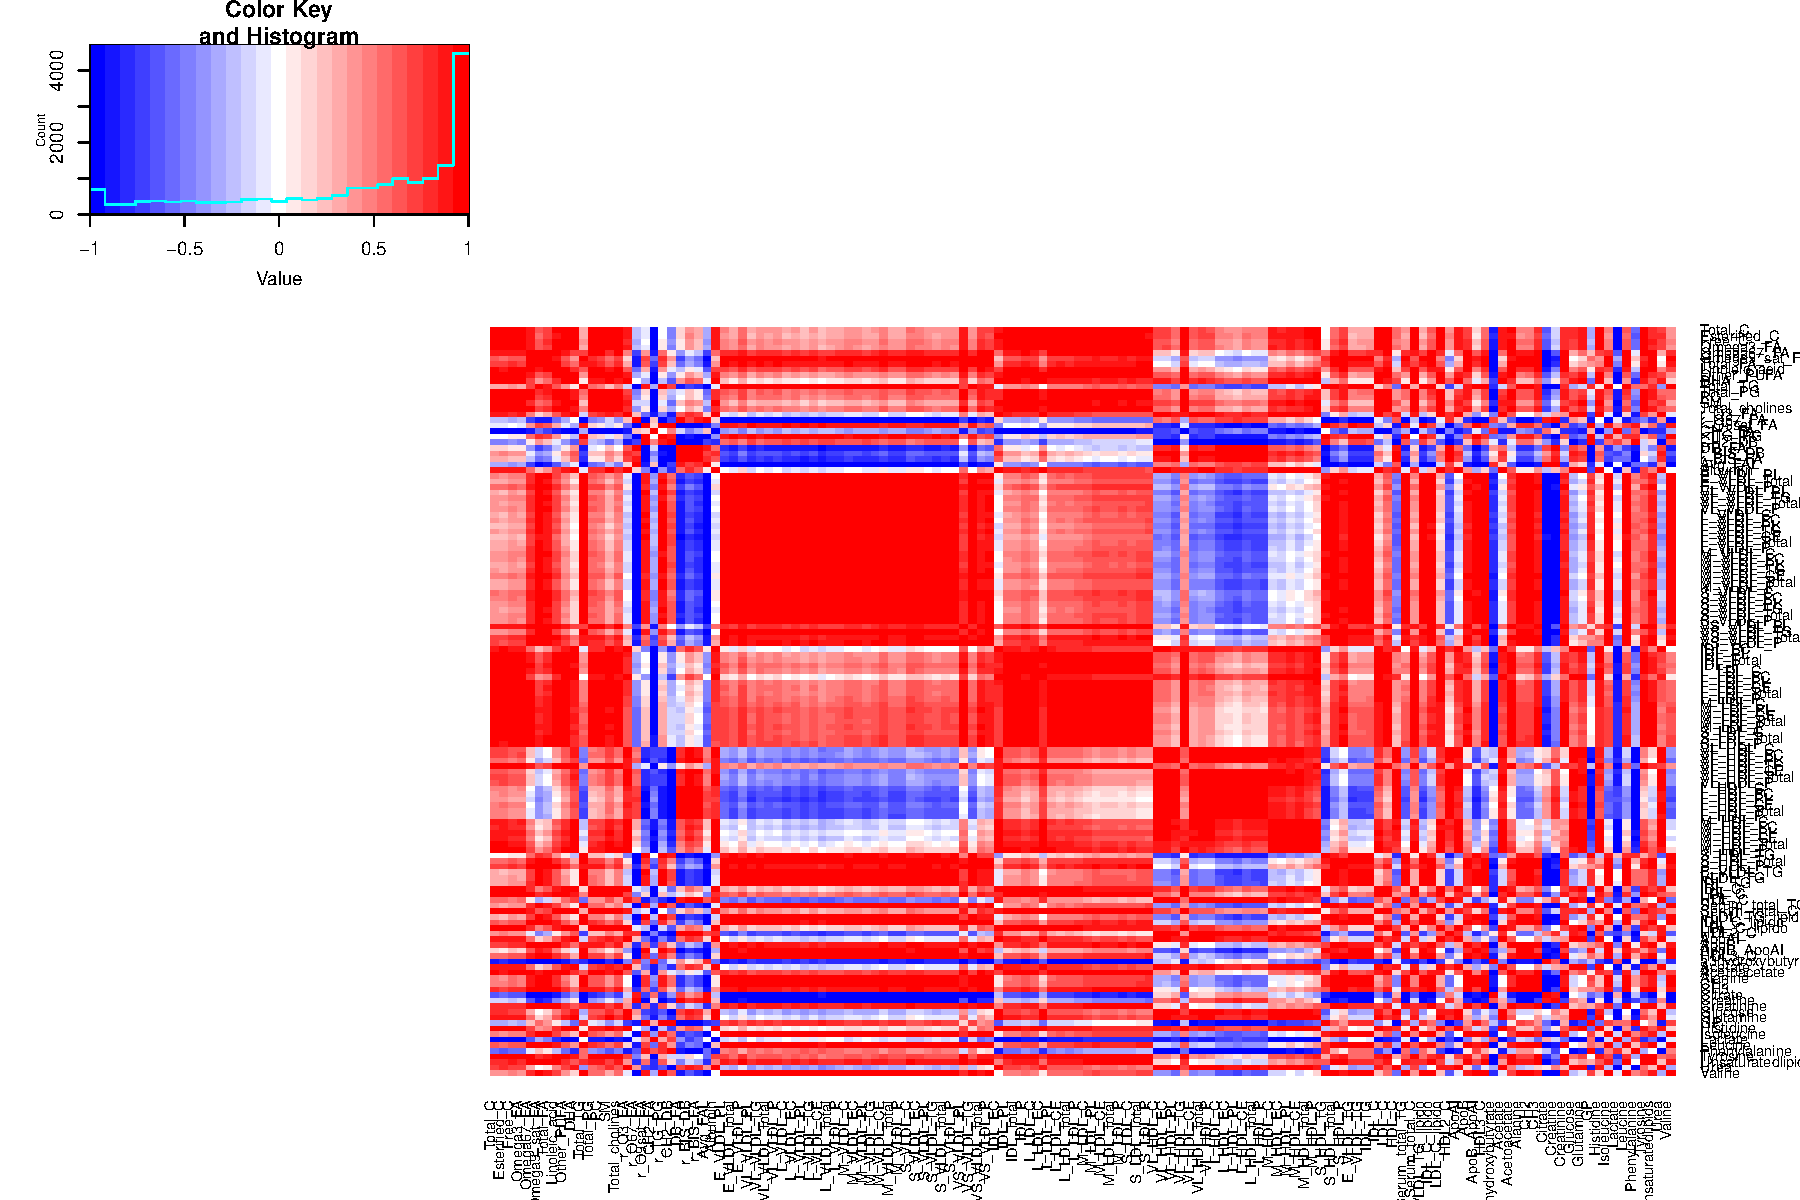
\includegraphics{Figs/Heatmap decomposition-1.pdf}

\begin{Shaded}
\begin{Highlighting}[]
\KeywordTok{hm.2}\NormalTok{(}\KeywordTok{cor}\NormalTok{(}\KeywordTok{with}\NormalTok{(fit,U_Xosc%*%}\KeywordTok{t}\NormalTok{(P_Xosc.))))}
\end{Highlighting}
\end{Shaded}

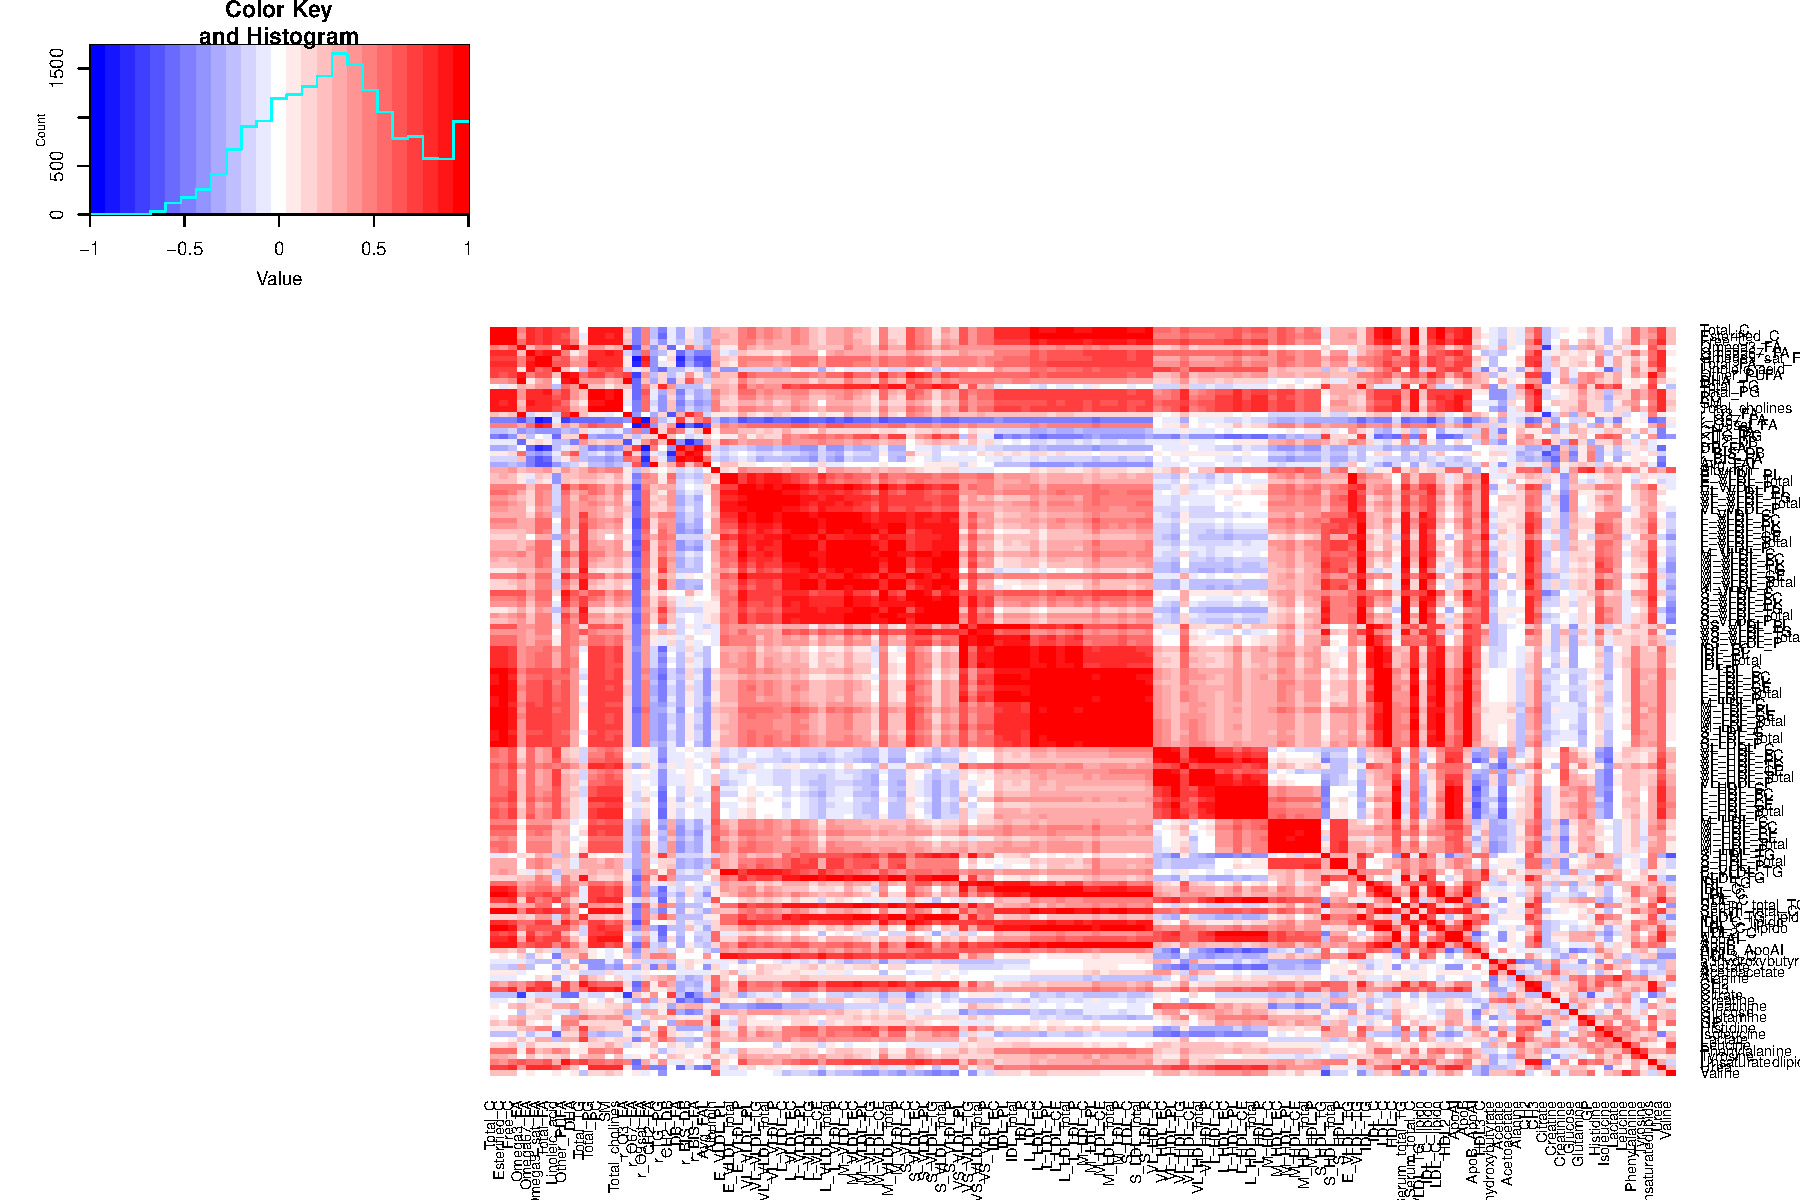
\includegraphics{Figs/Heatmap decomposition-2.pdf}

\begin{Shaded}
\begin{Highlighting}[]
\KeywordTok{hm.2}\NormalTok{(}\KeywordTok{cor}\NormalTok{(}\KeywordTok{with}\NormalTok{(fit,Ff)))}
\end{Highlighting}
\end{Shaded}

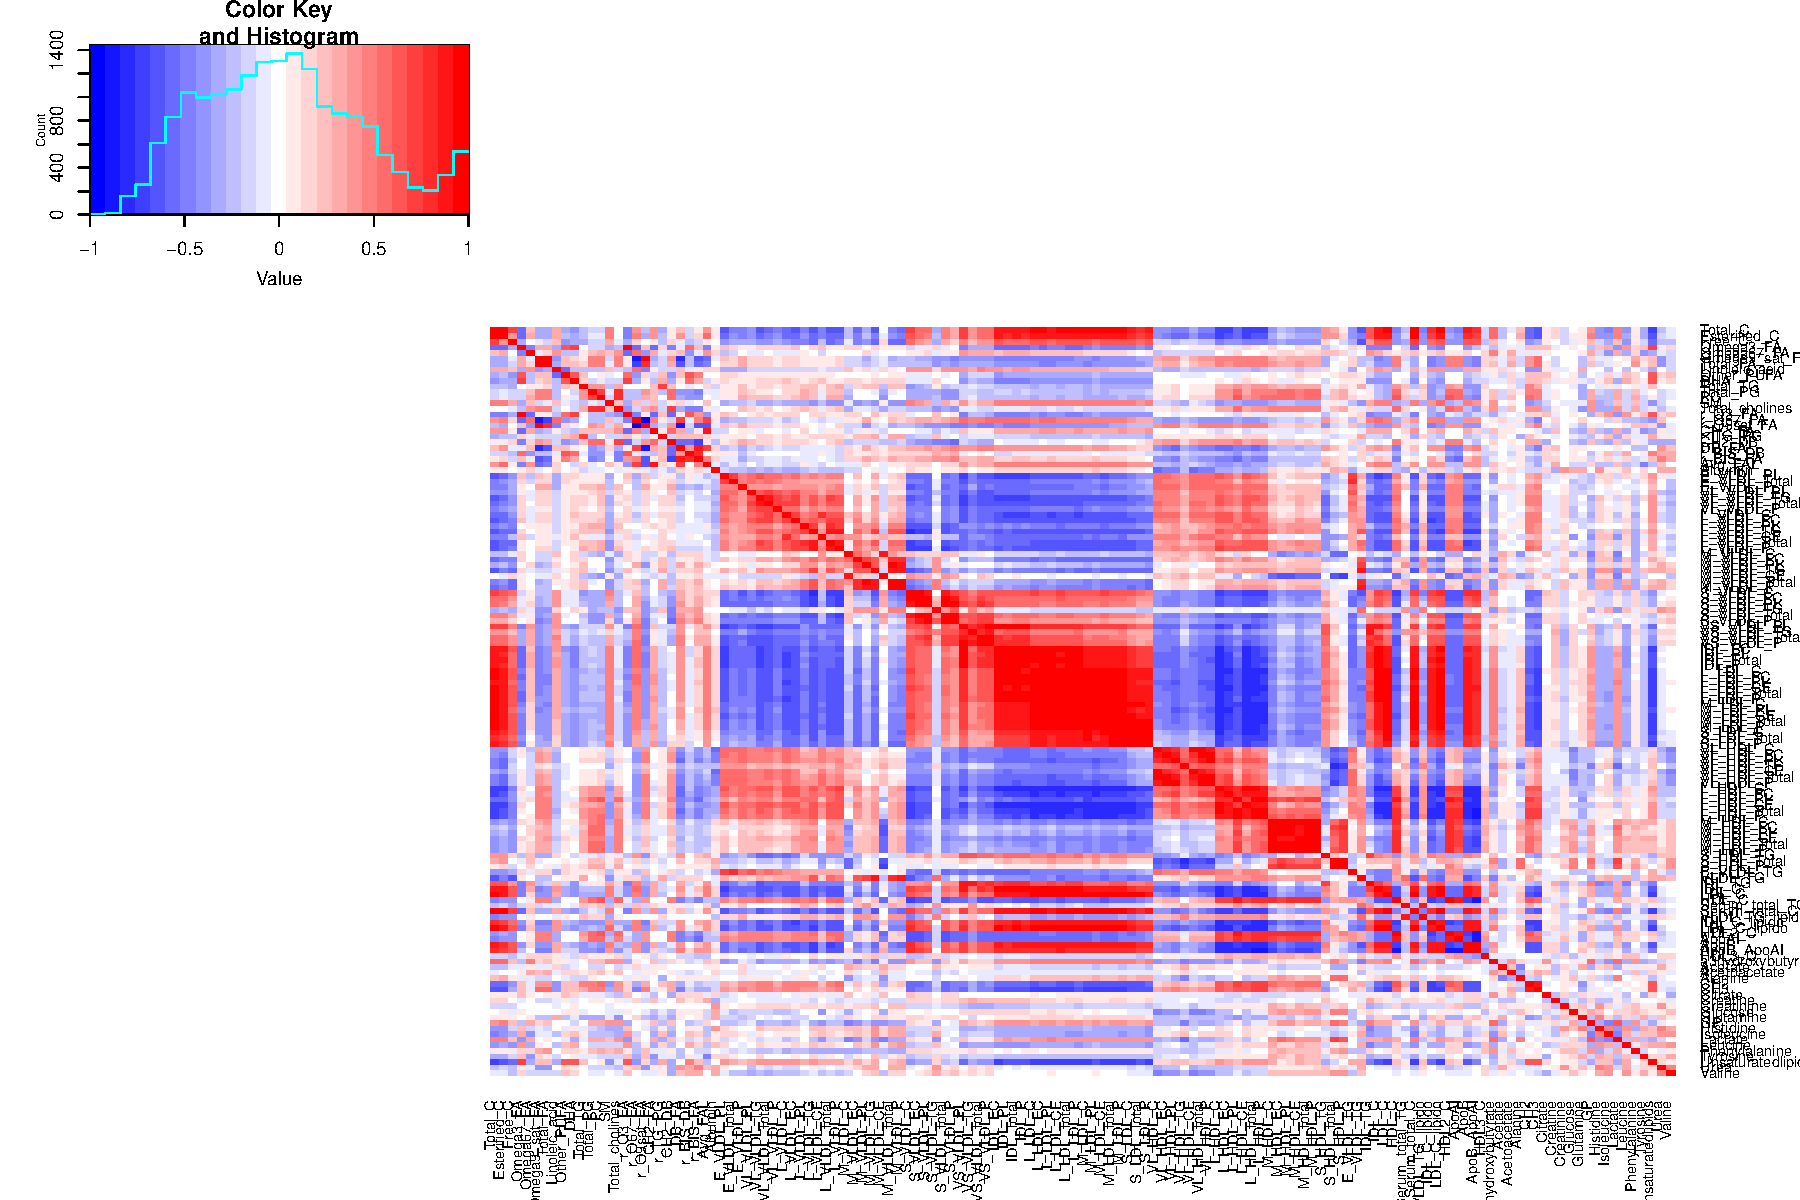
\includegraphics{Figs/Heatmap decomposition-3.pdf}

\subsubsection{CPU times}\label{cpu-times}

\textbf{Packages needed}

\begin{itemize}
\tightlist
\item
  \texttt{install.packages("microbenchmark")}
\end{itemize}

In OmicsPLS we added an alternative, memory-efficient, fitting algorithm
(NIPALS) for high-dimensional data. This omits storing the whole
covariance matrix of size \(p\) times \(q\). In case \(p\) and \(q\) are
large, say larger than 3000 both, storing this becomes a memory
intensive operation. To see how long \texttt{o2m} takes to fit, we
consider three scenarios. They are timed with the
\texttt{microbenchmark} function.

\begin{Shaded}
\begin{Highlighting}[]
\KeywordTok{set.seed}\NormalTok{(}\DecValTok{2016}\NormalTok{^}\DecValTok{2}\NormalTok{)}
\NormalTok{fake_X <-}\StringTok{ }\KeywordTok{scale}\NormalTok{(}\KeywordTok{matrix}\NormalTok{(}\KeywordTok{rnorm}\NormalTok{(}\FloatTok{1e2}\NormalTok{*}\FloatTok{1e4}\NormalTok{),}\FloatTok{1e2}\NormalTok{))}
\NormalTok{fake_Y <-}\StringTok{ }\KeywordTok{scale}\NormalTok{(}\KeywordTok{matrix}\NormalTok{(}\KeywordTok{rnorm}\NormalTok{(}\FloatTok{1e2}\NormalTok{*}\FloatTok{1e2}\NormalTok{),}\FloatTok{1e2}\NormalTok{))}
\KeywordTok{suppressMessages}\NormalTok{(}
  \NormalTok{scenario1 <-}\StringTok{ }\NormalTok{microbenchmark::}\KeywordTok{microbenchmark}\NormalTok{(}
    \DataTypeTok{default=}\KeywordTok{o2m}\NormalTok{(fake_X, fake_Y, }\DecValTok{1}\NormalTok{, }\DecValTok{1}\NormalTok{, }\DecValTok{1}\NormalTok{),}
    \DataTypeTok{stripped=}\KeywordTok{o2m}\NormalTok{(fake_X, fake_Y, }\DecValTok{1}\NormalTok{, }\DecValTok{1}\NormalTok{, }\DecValTok{1}\NormalTok{, }\DataTypeTok{stripped=}\NormalTok{T),}
    \DataTypeTok{highD =} \KeywordTok{o2m}\NormalTok{(fake_X, fake_Y, }\DecValTok{1}\NormalTok{, }\DecValTok{1}\NormalTok{, }\DecValTok{1}\NormalTok{, }\DataTypeTok{stripped=}\NormalTok{T, }\DataTypeTok{p_thresh=}\DecValTok{1}\NormalTok{),}
    \DataTypeTok{times =} \DecValTok{5}\NormalTok{, }\DataTypeTok{unit =} \StringTok{'s'}\NormalTok{,}\DataTypeTok{control=}\KeywordTok{list}\NormalTok{(}\DataTypeTok{warmup=}\DecValTok{1}\NormalTok{))}
\NormalTok{)}

\NormalTok{fake_X <-}\StringTok{ }\KeywordTok{scale}\NormalTok{(}\KeywordTok{matrix}\NormalTok{(}\KeywordTok{rnorm}\NormalTok{(}\FloatTok{1e2}\NormalTok{*}\FloatTok{2e3}\NormalTok{),}\FloatTok{1e2}\NormalTok{))}
\NormalTok{fake_Y <-}\StringTok{ }\KeywordTok{scale}\NormalTok{(}\KeywordTok{matrix}\NormalTok{(}\KeywordTok{rnorm}\NormalTok{(}\FloatTok{1e2}\NormalTok{*}\FloatTok{2e3}\NormalTok{),}\FloatTok{1e2}\NormalTok{))}
\KeywordTok{suppressMessages}\NormalTok{(}
  \NormalTok{scenario2 <-}\StringTok{ }\NormalTok{microbenchmark::}\KeywordTok{microbenchmark}\NormalTok{(}
    \DataTypeTok{default=}\KeywordTok{o2m}\NormalTok{(fake_X, fake_Y, }\DecValTok{1}\NormalTok{, }\DecValTok{1}\NormalTok{, }\DecValTok{1}\NormalTok{),}
    \DataTypeTok{stripped=}\KeywordTok{o2m}\NormalTok{(fake_X, fake_Y, }\DecValTok{1}\NormalTok{, }\DecValTok{1}\NormalTok{, }\DecValTok{1}\NormalTok{, }\DataTypeTok{stripped=}\NormalTok{T),}
    \DataTypeTok{highD =} \KeywordTok{o2m}\NormalTok{(fake_X, fake_Y, }\DecValTok{1}\NormalTok{, }\DecValTok{1}\NormalTok{, }\DecValTok{1}\NormalTok{, }\DataTypeTok{stripped=}\NormalTok{T, }\DataTypeTok{p_thresh=}\DecValTok{1}\NormalTok{),}
    \DataTypeTok{times =} \DecValTok{5}\NormalTok{, }\DataTypeTok{unit =} \StringTok{'s'}\NormalTok{,}\DataTypeTok{control=}\KeywordTok{list}\NormalTok{(}\DataTypeTok{warmup=}\DecValTok{1}\NormalTok{))}
\NormalTok{)}

\NormalTok{fake_X <-}\StringTok{ }\KeywordTok{scale}\NormalTok{(}\KeywordTok{matrix}\NormalTok{(}\KeywordTok{rnorm}\NormalTok{(}\FloatTok{1e2}\NormalTok{*}\FloatTok{5e4}\NormalTok{),}\FloatTok{1e2}\NormalTok{))}
\NormalTok{fake_Y <-}\StringTok{ }\KeywordTok{scale}\NormalTok{(}\KeywordTok{matrix}\NormalTok{(}\KeywordTok{rnorm}\NormalTok{(}\FloatTok{1e2}\NormalTok{*}\FloatTok{5e4}\NormalTok{),}\FloatTok{1e2}\NormalTok{))}
\KeywordTok{try}\NormalTok{(}\KeywordTok{o2m}\NormalTok{(fake_X, fake_Y, }\DecValTok{1}\NormalTok{, }\DecValTok{1}\NormalTok{, }\DecValTok{1}\NormalTok{, }\DataTypeTok{p_thresh=}\FloatTok{1e6}\NormalTok{))}
\end{Highlighting}
\end{Shaded}

\begin{verbatim}
## Warning in as.matrix(x): Reached total allocation of 8096Mb: see
## help(memory.size)

## Warning in as.matrix(x): Reached total allocation of 8096Mb: see
## help(memory.size)

## Warning in as.matrix(x): Reached total allocation of 8096Mb: see
## help(memory.size)

## Warning in as.matrix(x): Reached total allocation of 8096Mb: see
## help(memory.size)
\end{verbatim}

\begin{Shaded}
\begin{Highlighting}[]
\KeywordTok{try}\NormalTok{(}\KeywordTok{o2m}\NormalTok{(fake_X, fake_Y, }\DecValTok{1}\NormalTok{, }\DecValTok{1}\NormalTok{, }\DecValTok{1}\NormalTok{, }\DataTypeTok{stripped=}\NormalTok{T, }\DataTypeTok{p_thresh=}\FloatTok{1e6}\NormalTok{))}
\end{Highlighting}
\end{Shaded}

\begin{verbatim}
## Warning in as.matrix(x): Reached total allocation of 8096Mb: see
## help(memory.size)

## Warning in as.matrix(x): Reached total allocation of 8096Mb: see
## help(memory.size)

## Warning in as.matrix(x): Reached total allocation of 8096Mb: see
## help(memory.size)

## Warning in as.matrix(x): Reached total allocation of 8096Mb: see
## help(memory.size)
\end{verbatim}

\begin{Shaded}
\begin{Highlighting}[]
\KeywordTok{o2m}\NormalTok{(fake_X, fake_Y, }\DecValTok{1}\NormalTok{, }\DecValTok{1}\NormalTok{, }\DecValTok{1}\NormalTok{, }\DataTypeTok{stripped=}\NormalTok{T)}
\end{Highlighting}
\end{Shaded}

\begin{verbatim}
## Using Power Method with tolerance 1e-10 and max iterations 100
\end{verbatim}

\begin{verbatim}
## Power Method (comp 1) stopped after 100 iterations.
\end{verbatim}

\begin{verbatim}
## Power Method (comp 2) stopped after 100 iterations.
\end{verbatim}

\begin{verbatim}
## Power Method (comp 1) stopped after 100 iterations.
\end{verbatim}

\begin{verbatim}
## O2PLS fit: Stripped 
## with 1 joint components  
## and  1 orthogonal components in X 
## and  1 orthogonal components in Y 
## Elapsed time: 14.35 sec
\end{verbatim}

\begin{Shaded}
\begin{Highlighting}[]
\KeywordTok{rm}\NormalTok{(fake_X)}
\KeywordTok{rm}\NormalTok{(fake_Y)}
\end{Highlighting}
\end{Shaded}


\end{document}
